\section{Results}


\begin{figure}
\centering
 \subfloat{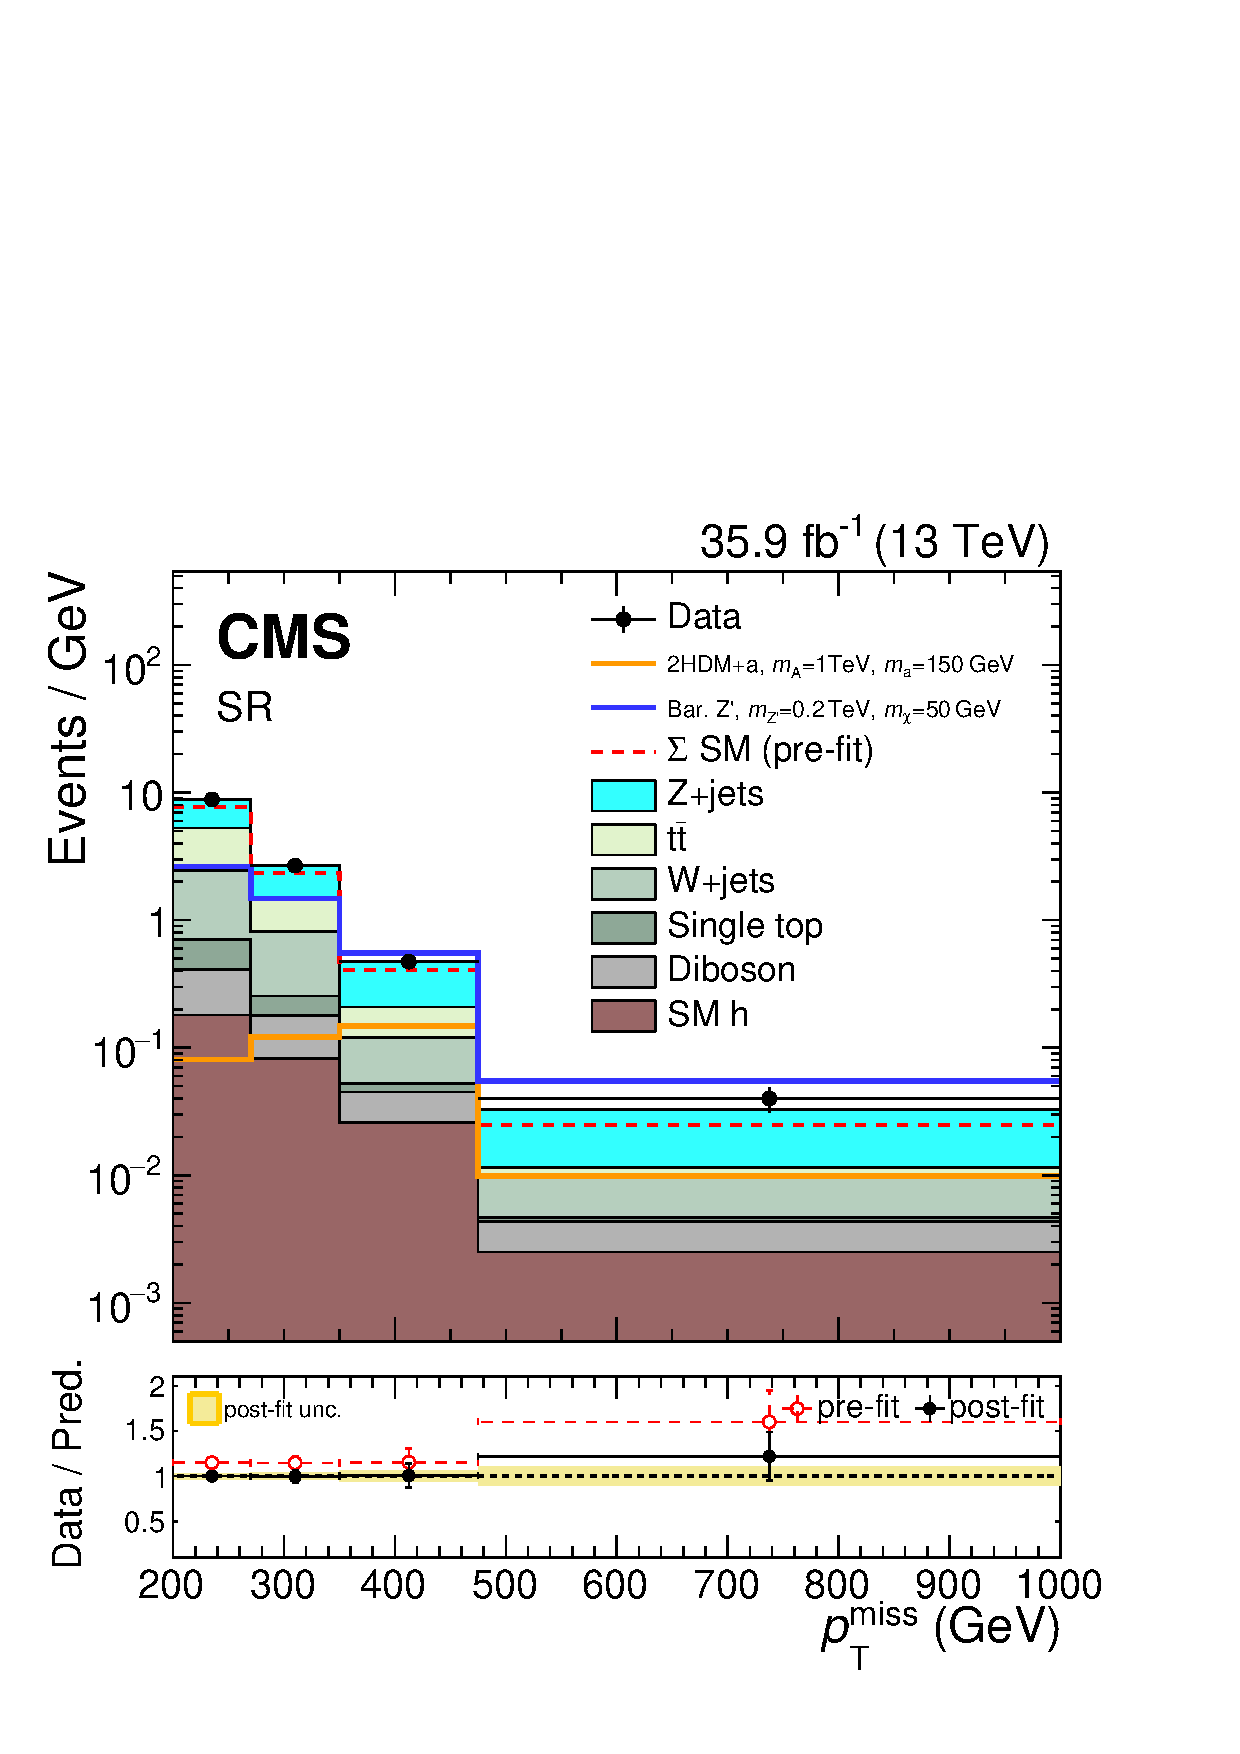
\includegraphics[width=0.45\textwidth]{figures/dataMC/MSDcorr_stackedPostfit_signal.pdf}}
% \subfloat{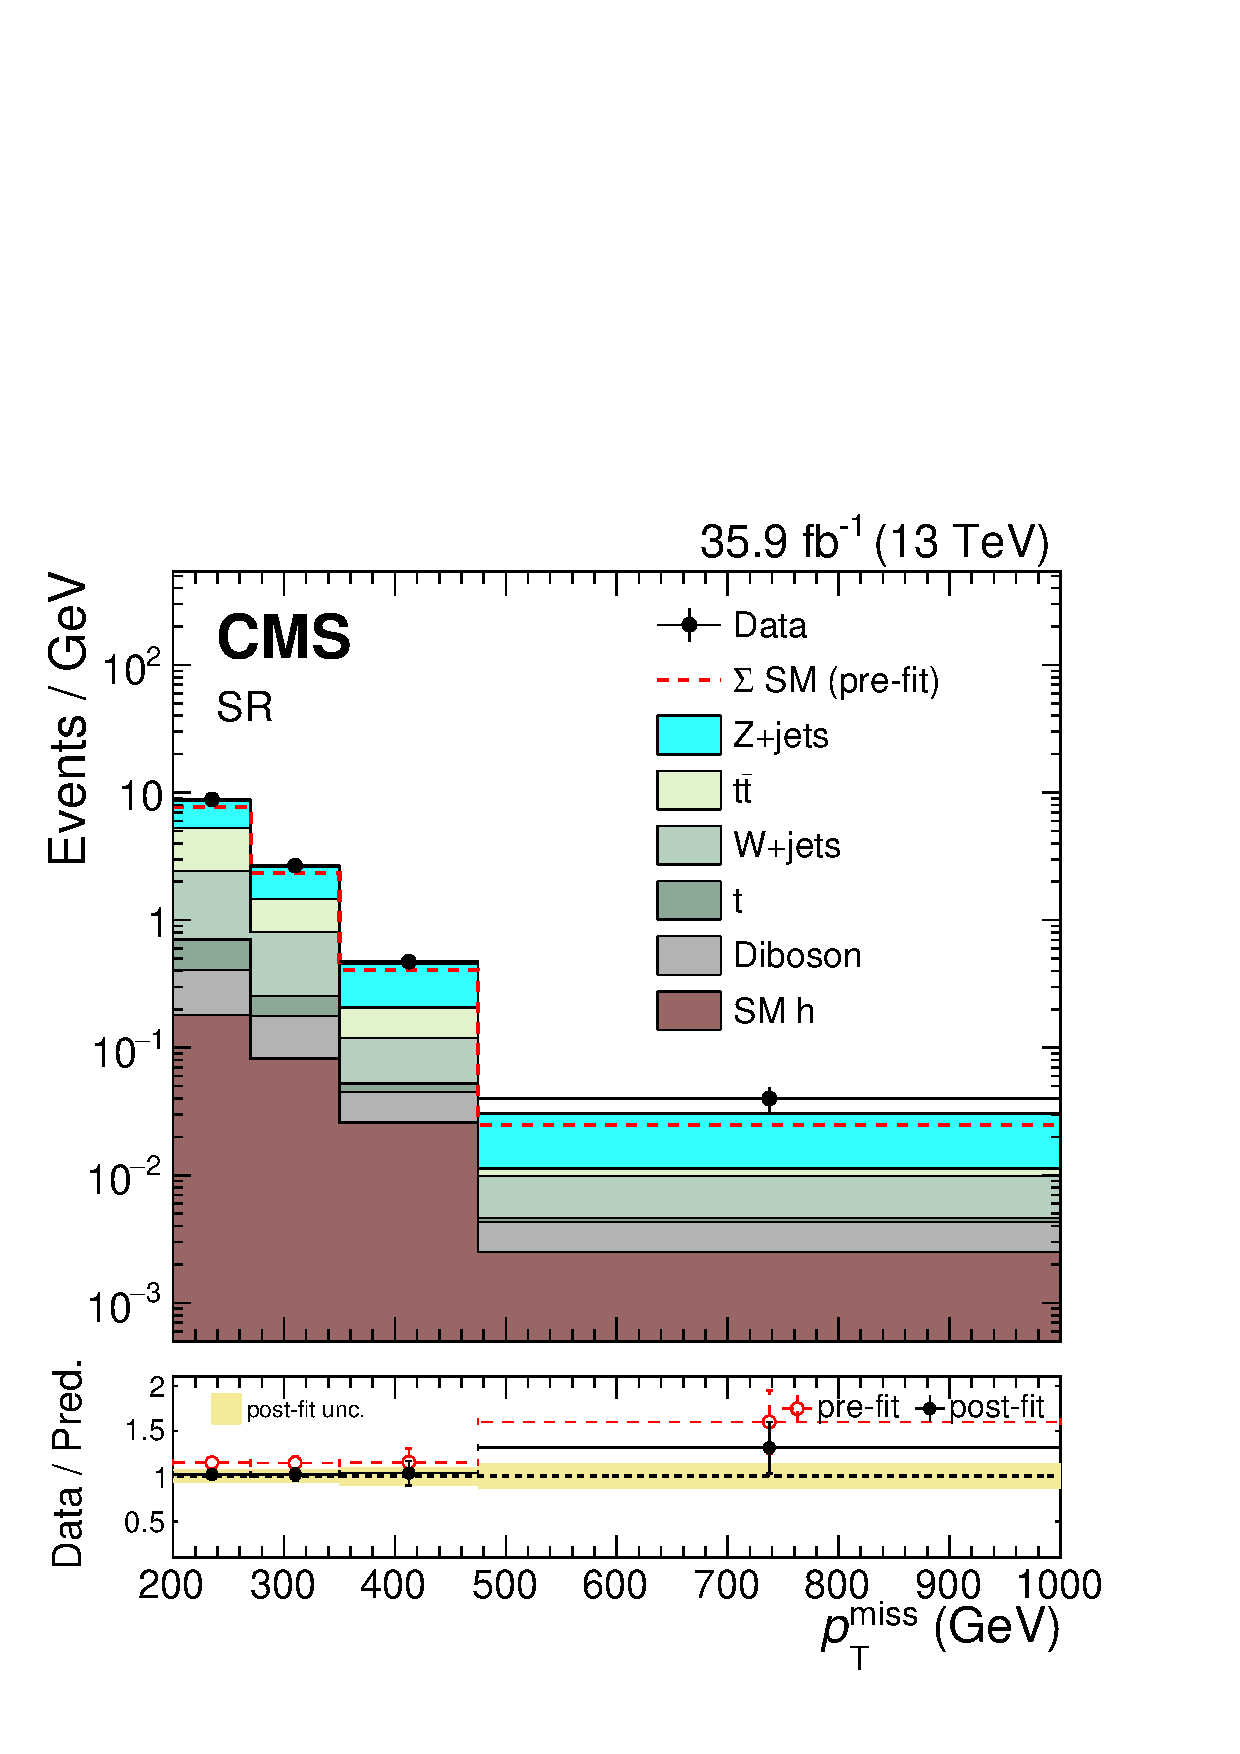
\includegraphics[width=0.45\textwidth]{figures/dataMC/MSDcorr_stackedPostfit_signal_masked.pdf}} \\
\caption{The \MET distribution in the signal region after a likelihood fit including the data in the signal region. The data are in agreement with post-fit background predictions for the SM backgrounds, and no significant excess is observed. The red histogram corresponds to the pre-fit estimate for the SM backgrounds.}
\label{Fig_sr}
\end{figure}


The expected yields and their uncertainties for each background in the SR as determined in the likelihood fit under the background-only assumption are presented in Table~\ref{tab:eventYieldTable}, along with the observed data yields. The signal region data have been included in the likelihood fit.  Table~\ref{tab:eventYieldTable_masked} lists the yields for a fit masking the data in the signal region. Good agreement is observed between the predictions for the two cases. In some bins, the uncertainty on the background sum is smaller than the one on individual contributions like from Z+jets due to anti-correlations between background processes. Expected yields are also presented for two signal models. The selection efficiencies for the chosen points correspond to 5\% for the 2HDM+a model and, respectively, to 1\% for the Baryonic Z' model. %As expected from the branching ratio of the Z boson, the uncertainties in the yields for the Z+jets process are smaller for the case where the signal region data has been included in the fit.

Figure \ref{Fig_sr} shows the pre-fit and post-fit \MET distribution in the SR for all SM backgrounds, as well as the observed data distribution. The likelihood fit has been performed simultaneously in all analysis regions. The data agree with the background predictions at the one-standard-deviation level, and the post-fit estimate of the SM background is slightly larger than the pre-fit one. The distributions for $U$ in the CRs are presented in Figures~\ref{Fig_cr_1} and \ref{Fig_cr_2}.

\begin{figure}
\centering
 \subfloat{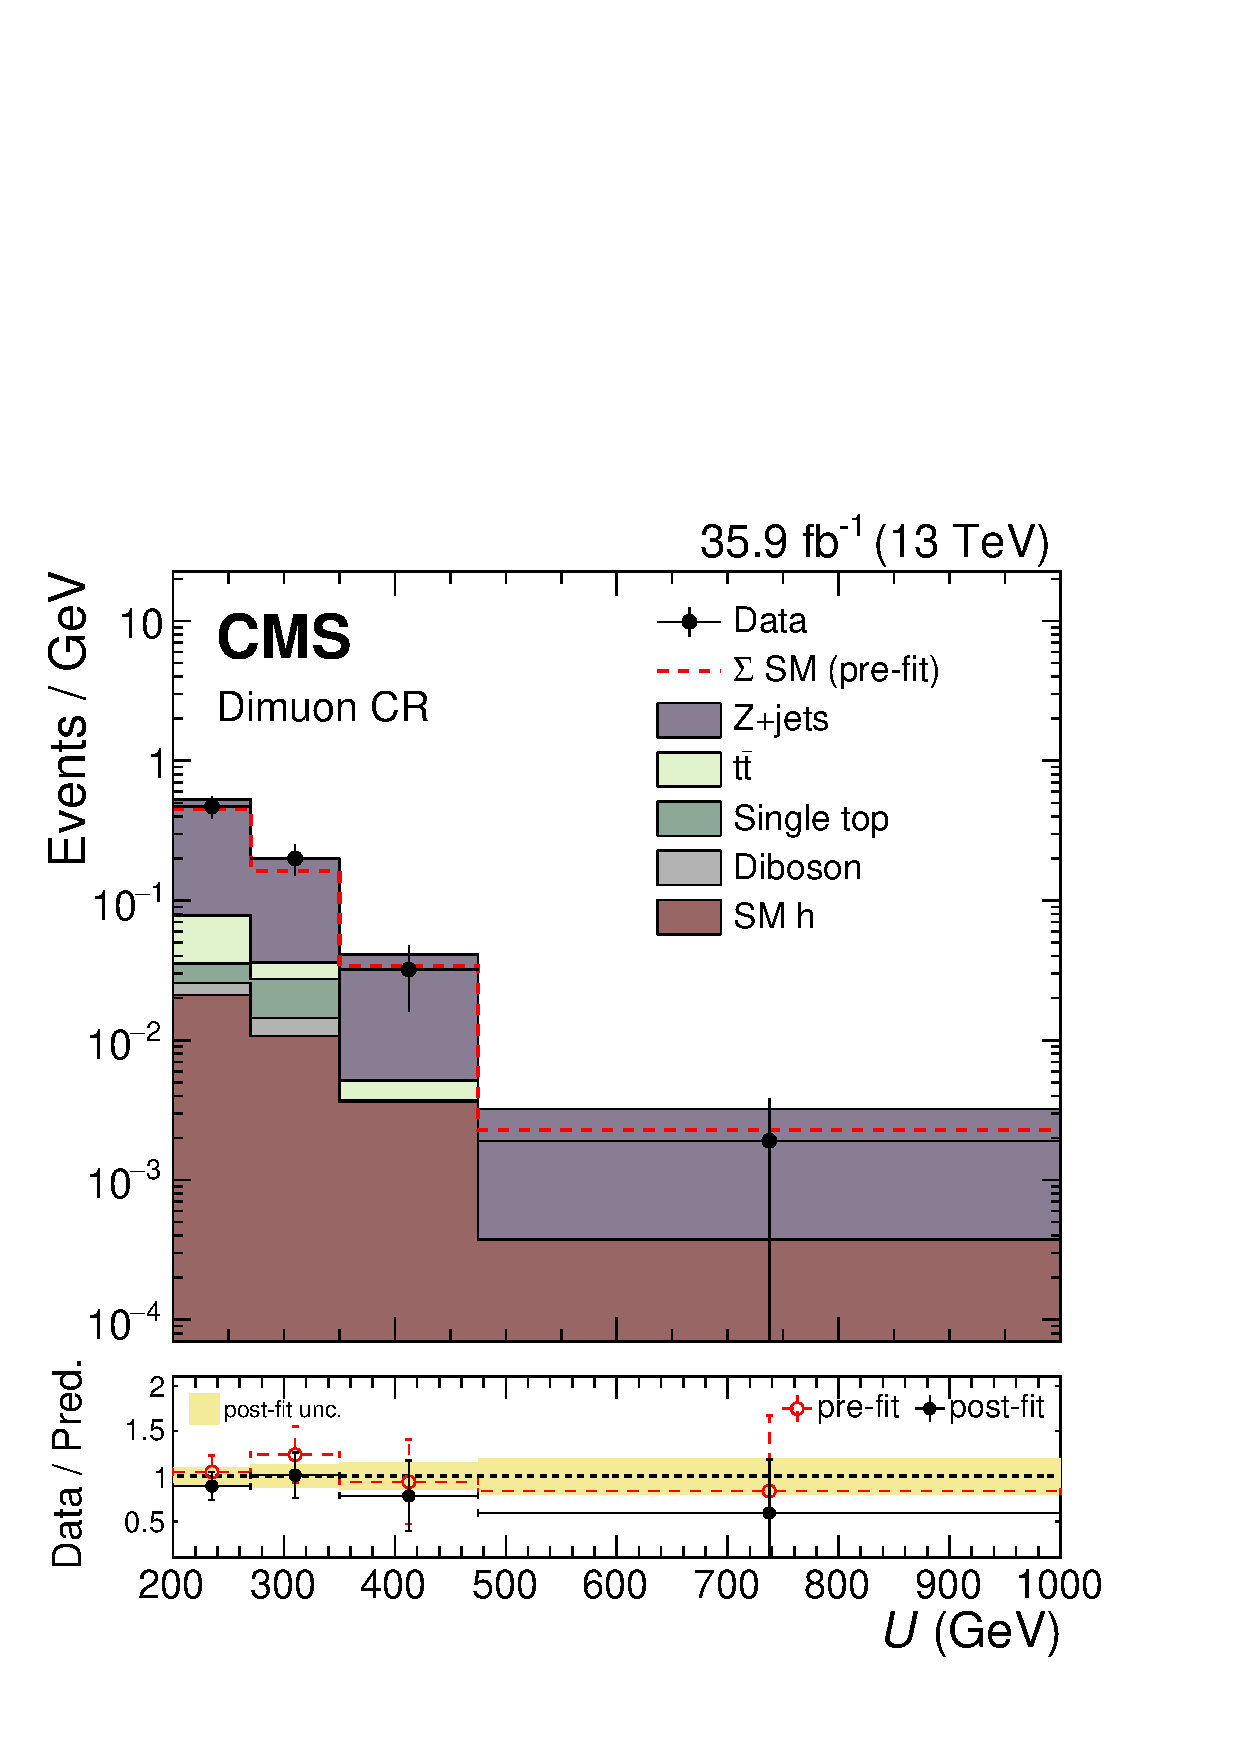
\includegraphics[width=0.36\textwidth]{figures/dataMC/MSDcorr_stackedPostfit_dimuon.pdf}}
 \subfloat{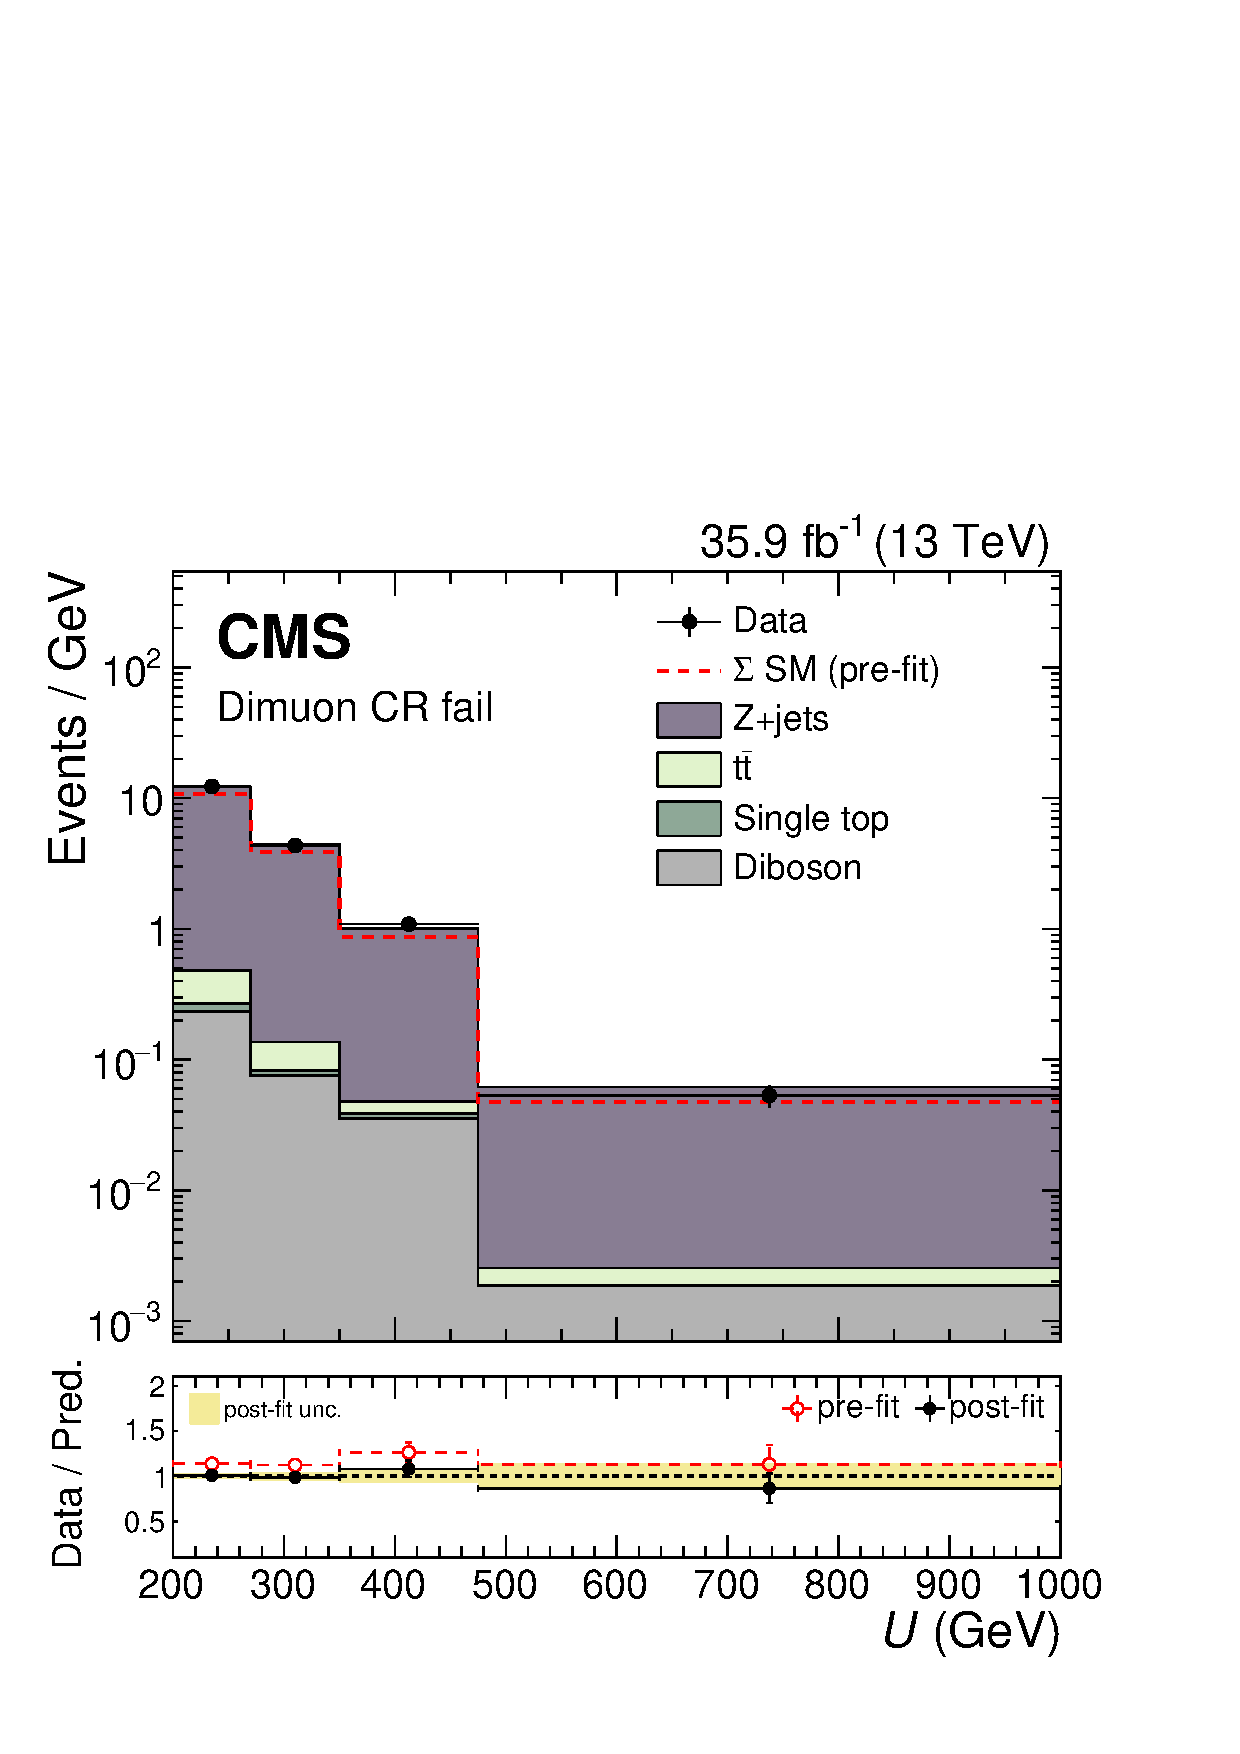
\includegraphics[width=0.36\textwidth]{figures/dataMC/MSDcorr_stackedPostfit_dimuon_fail.pdf}} \\
 \subfloat{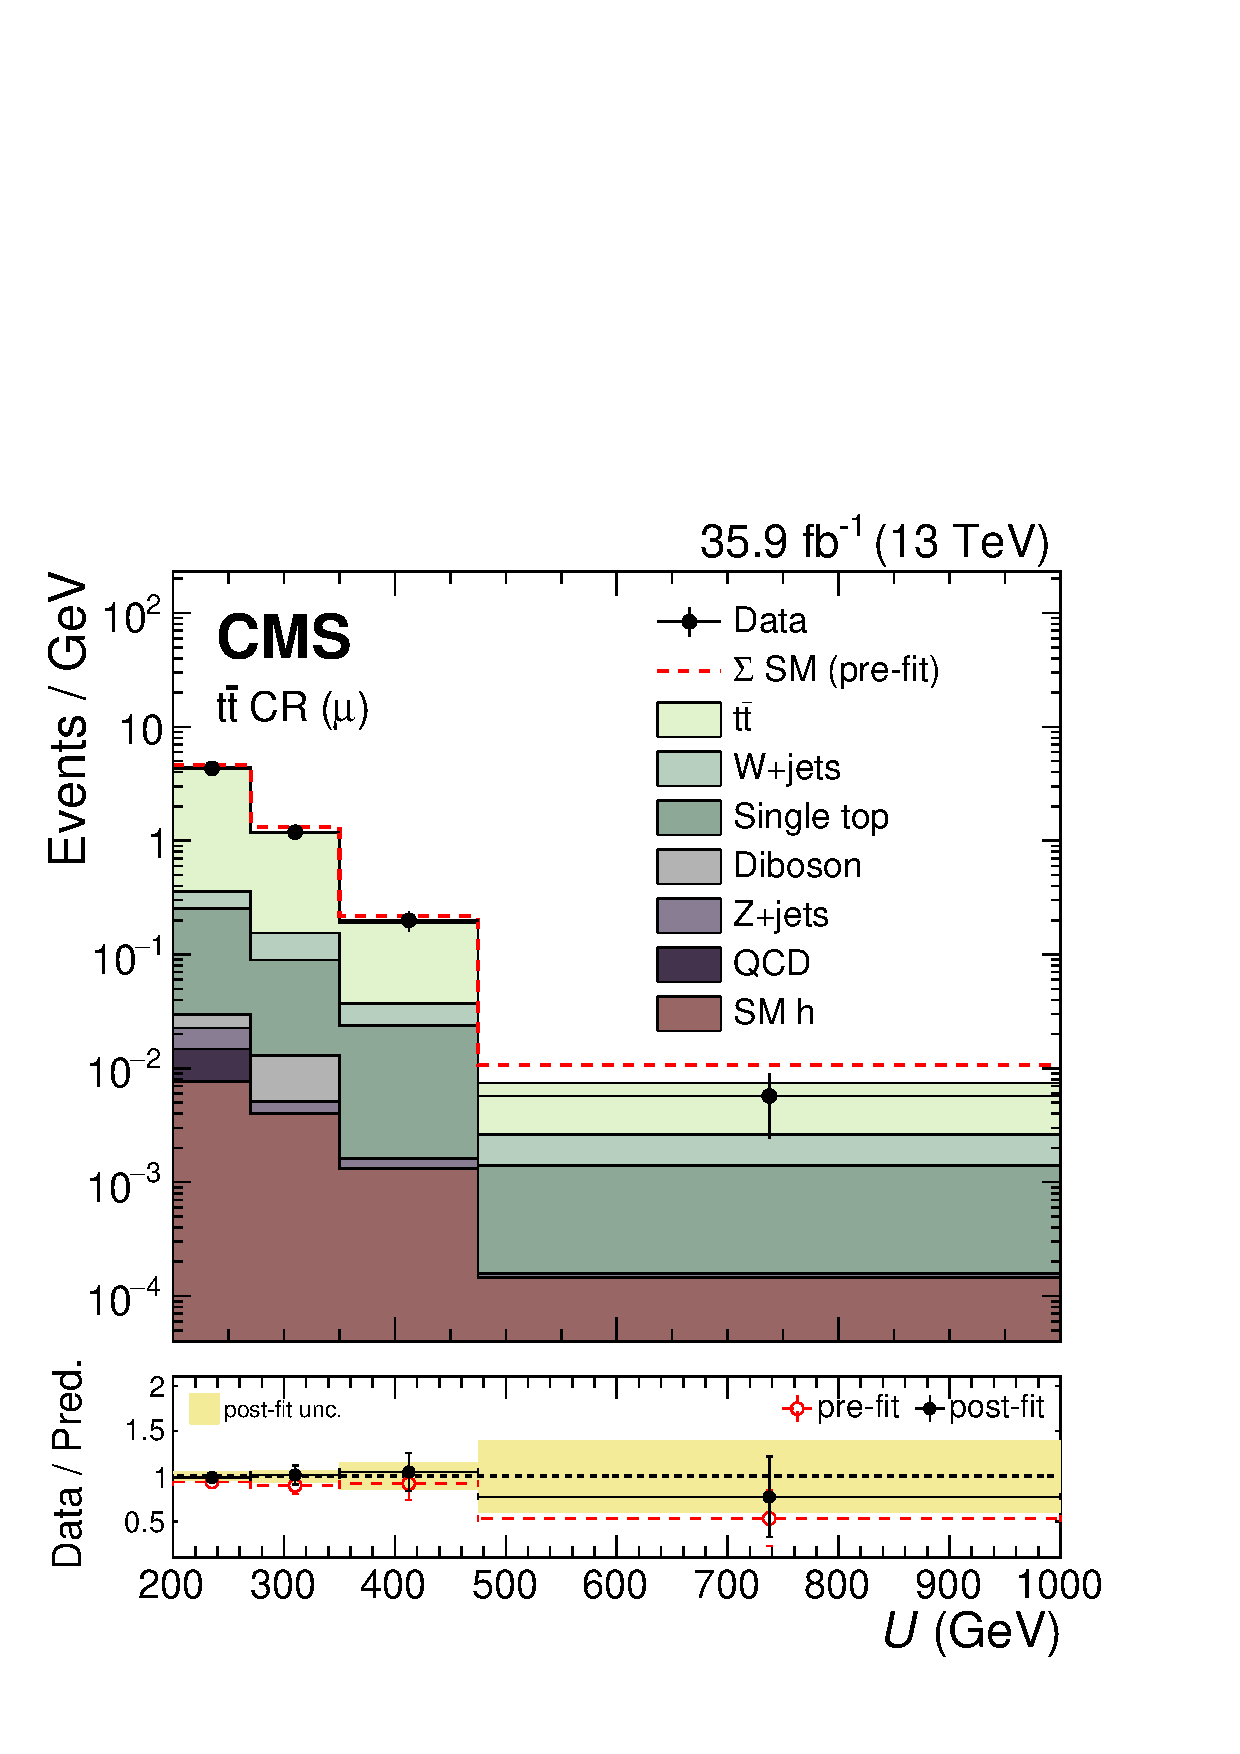
\includegraphics[width=0.36\textwidth]{figures/dataMC/MSDcorr_stackedPostfit_singlemuontop.pdf}}
 \subfloat{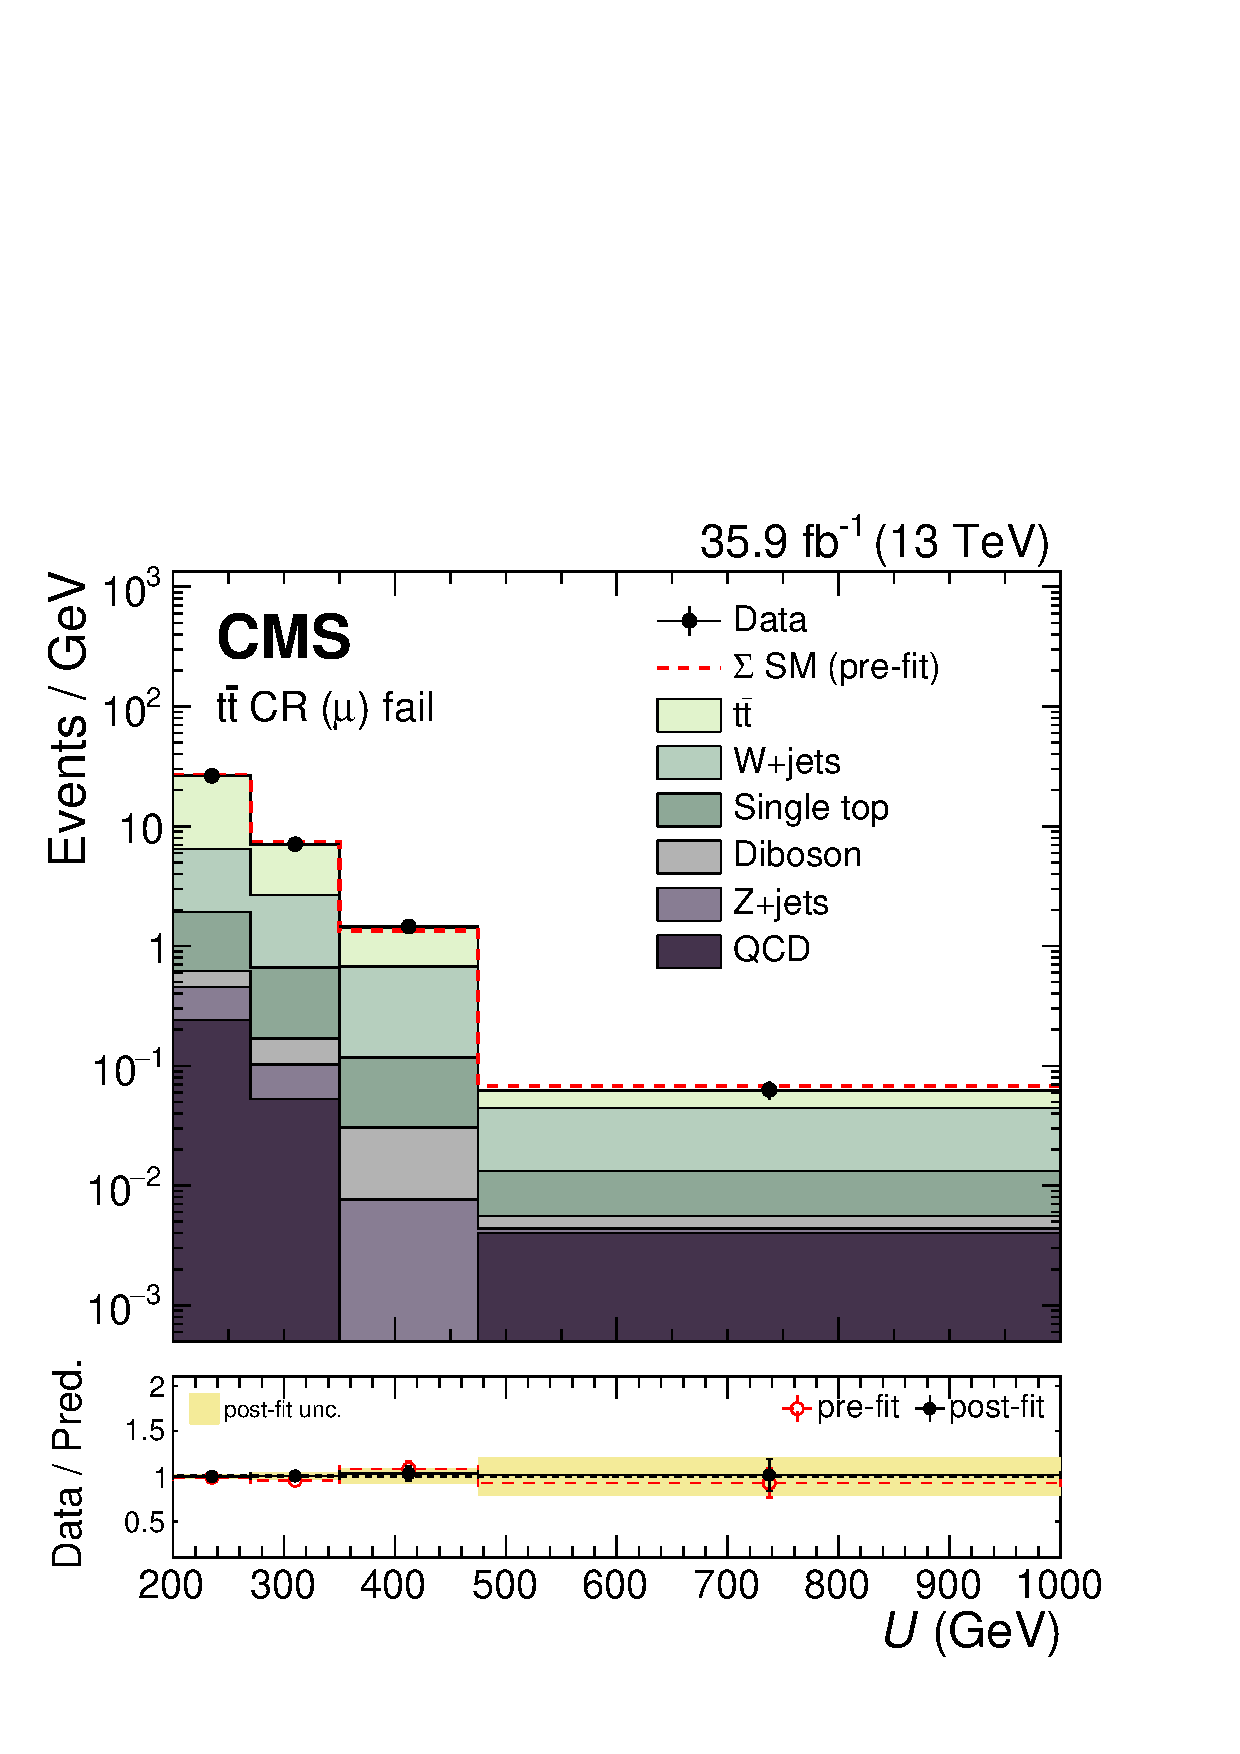
\includegraphics[width=0.36\textwidth]{figures/dataMC/MSDcorr_stackedPostfit_singlemuontop_fail.pdf}} \\
 \subfloat{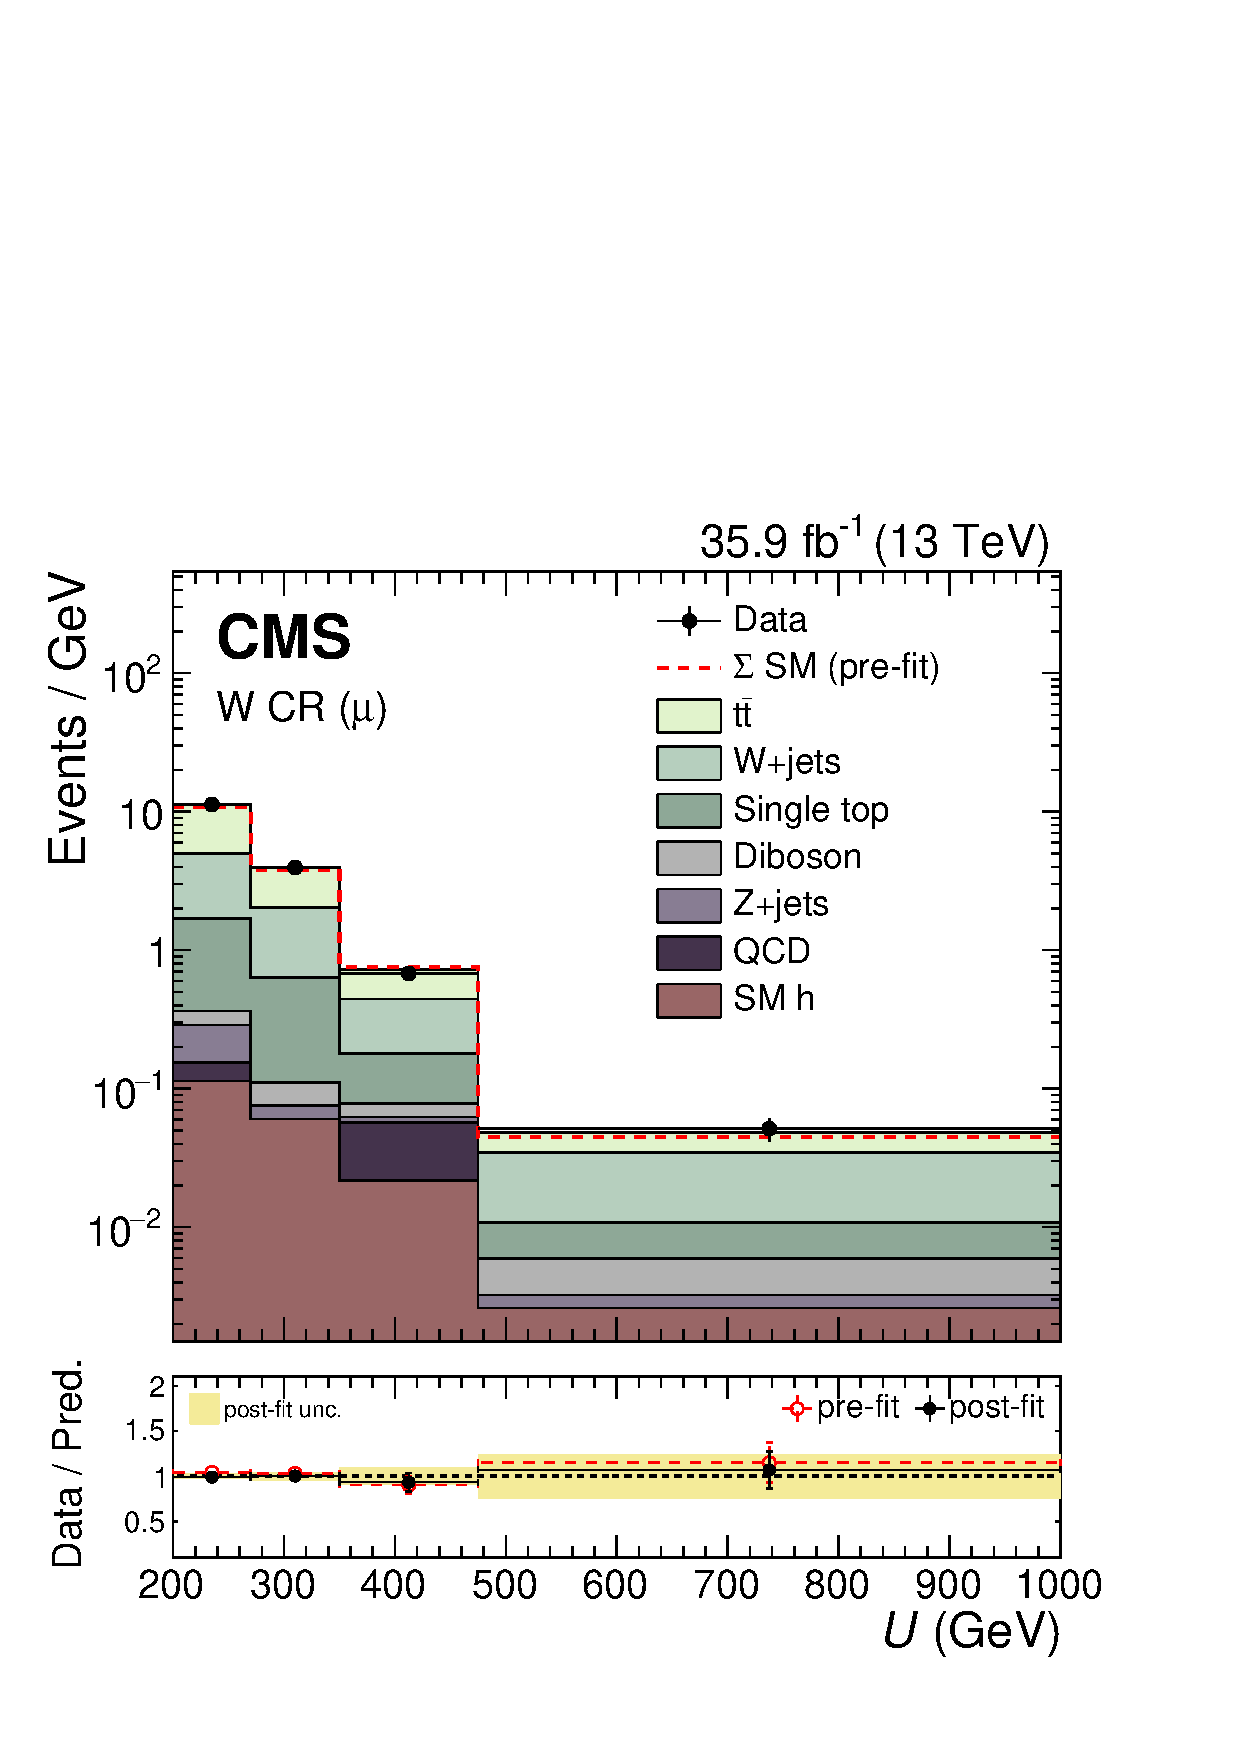
\includegraphics[width=0.36\textwidth]{figures/dataMC/MSDcorr_stackedPostfit_singlemuonw.pdf}}
 \subfloat{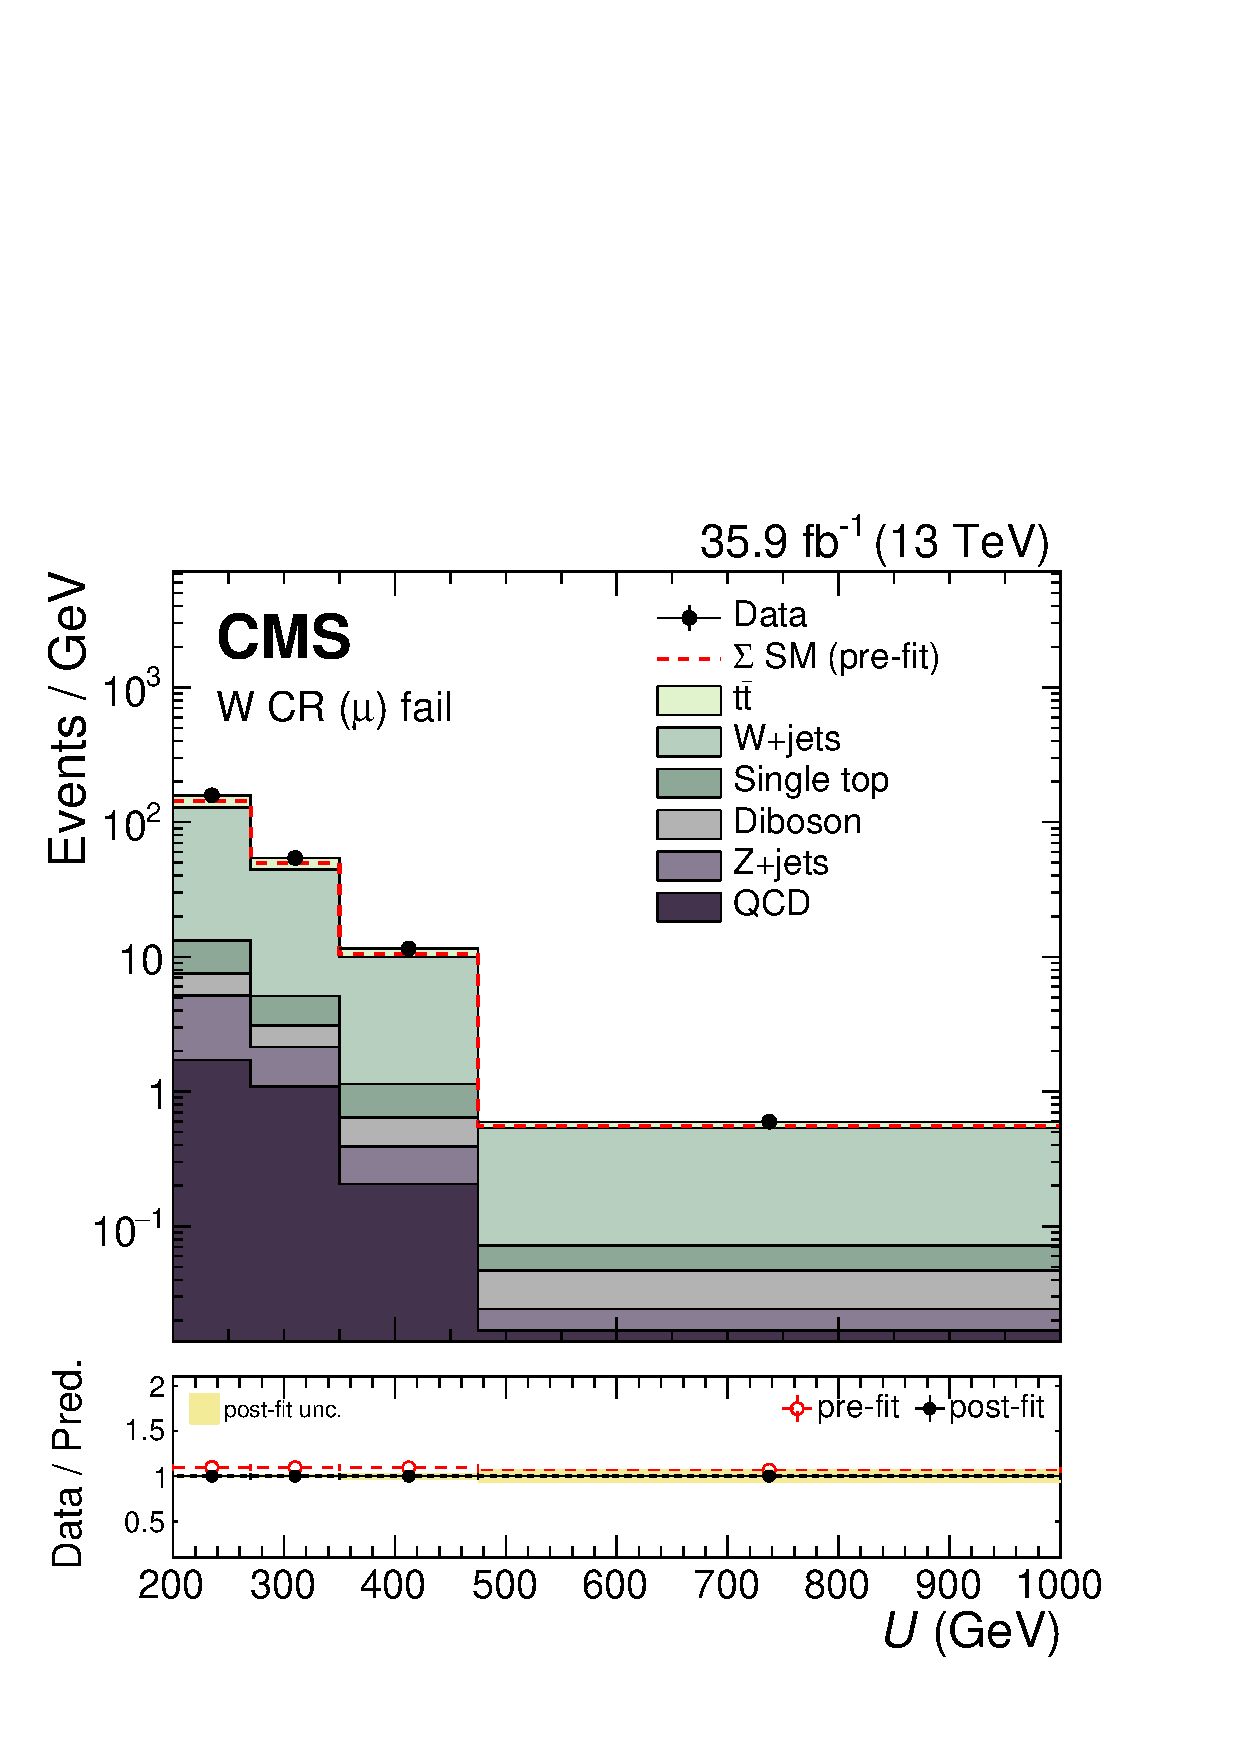
\includegraphics[width=0.36\textwidth]{figures/dataMC/MSDcorr_stackedPostfit_singlemuonw_fail.pdf}} \\
\caption{The $U$ distribution in the muon control regions after a fit to data, including the data in the signal region in the likelihood. Samples in the left distributions are selected with a passing requirement on the double-b tagger; a failing requirement is applied in the distributions to the right.}
\label{Fig_cr_1}
\end{figure}

\begin{figure}
\centering
 \subfloat{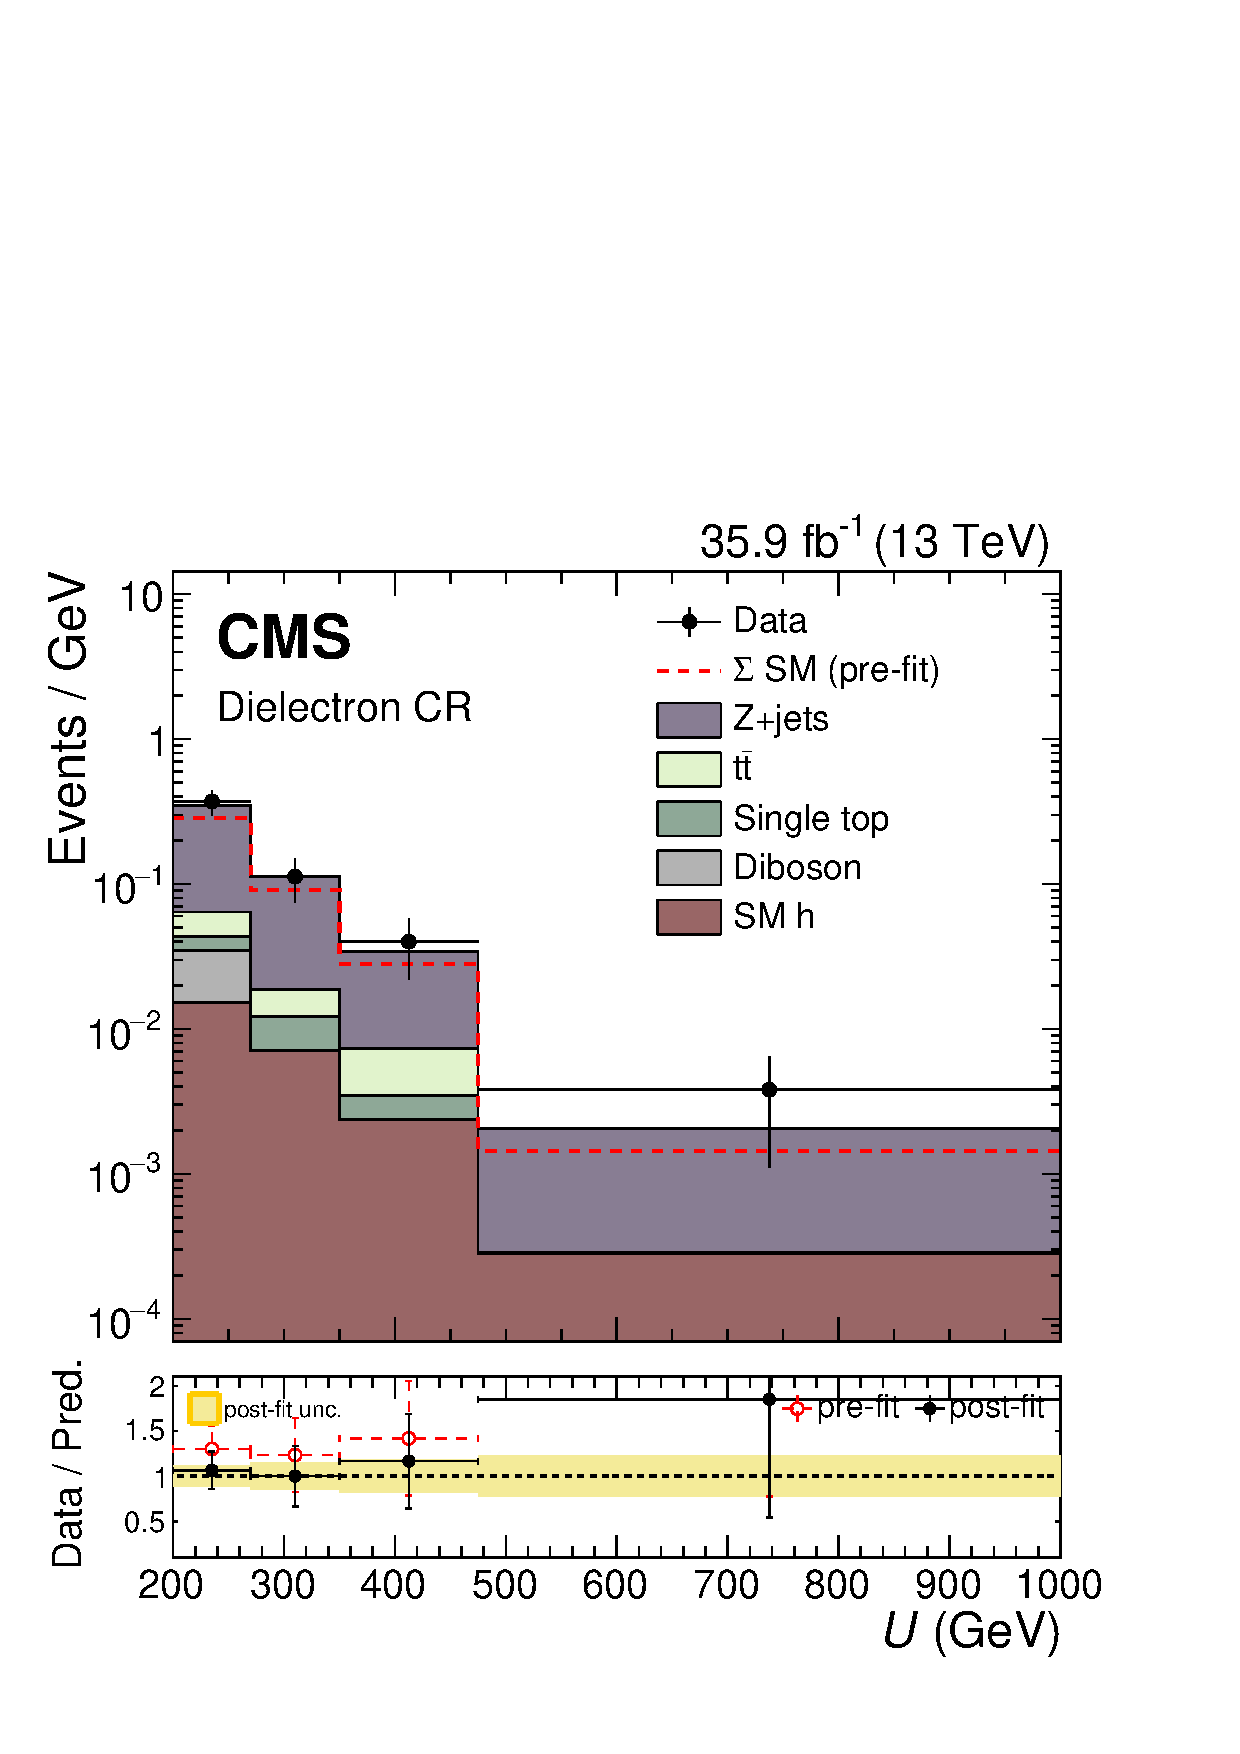
\includegraphics[width=0.36\textwidth]{figures/dataMC/MSDcorr_stackedPostfit_dielectron.pdf}}
 \subfloat{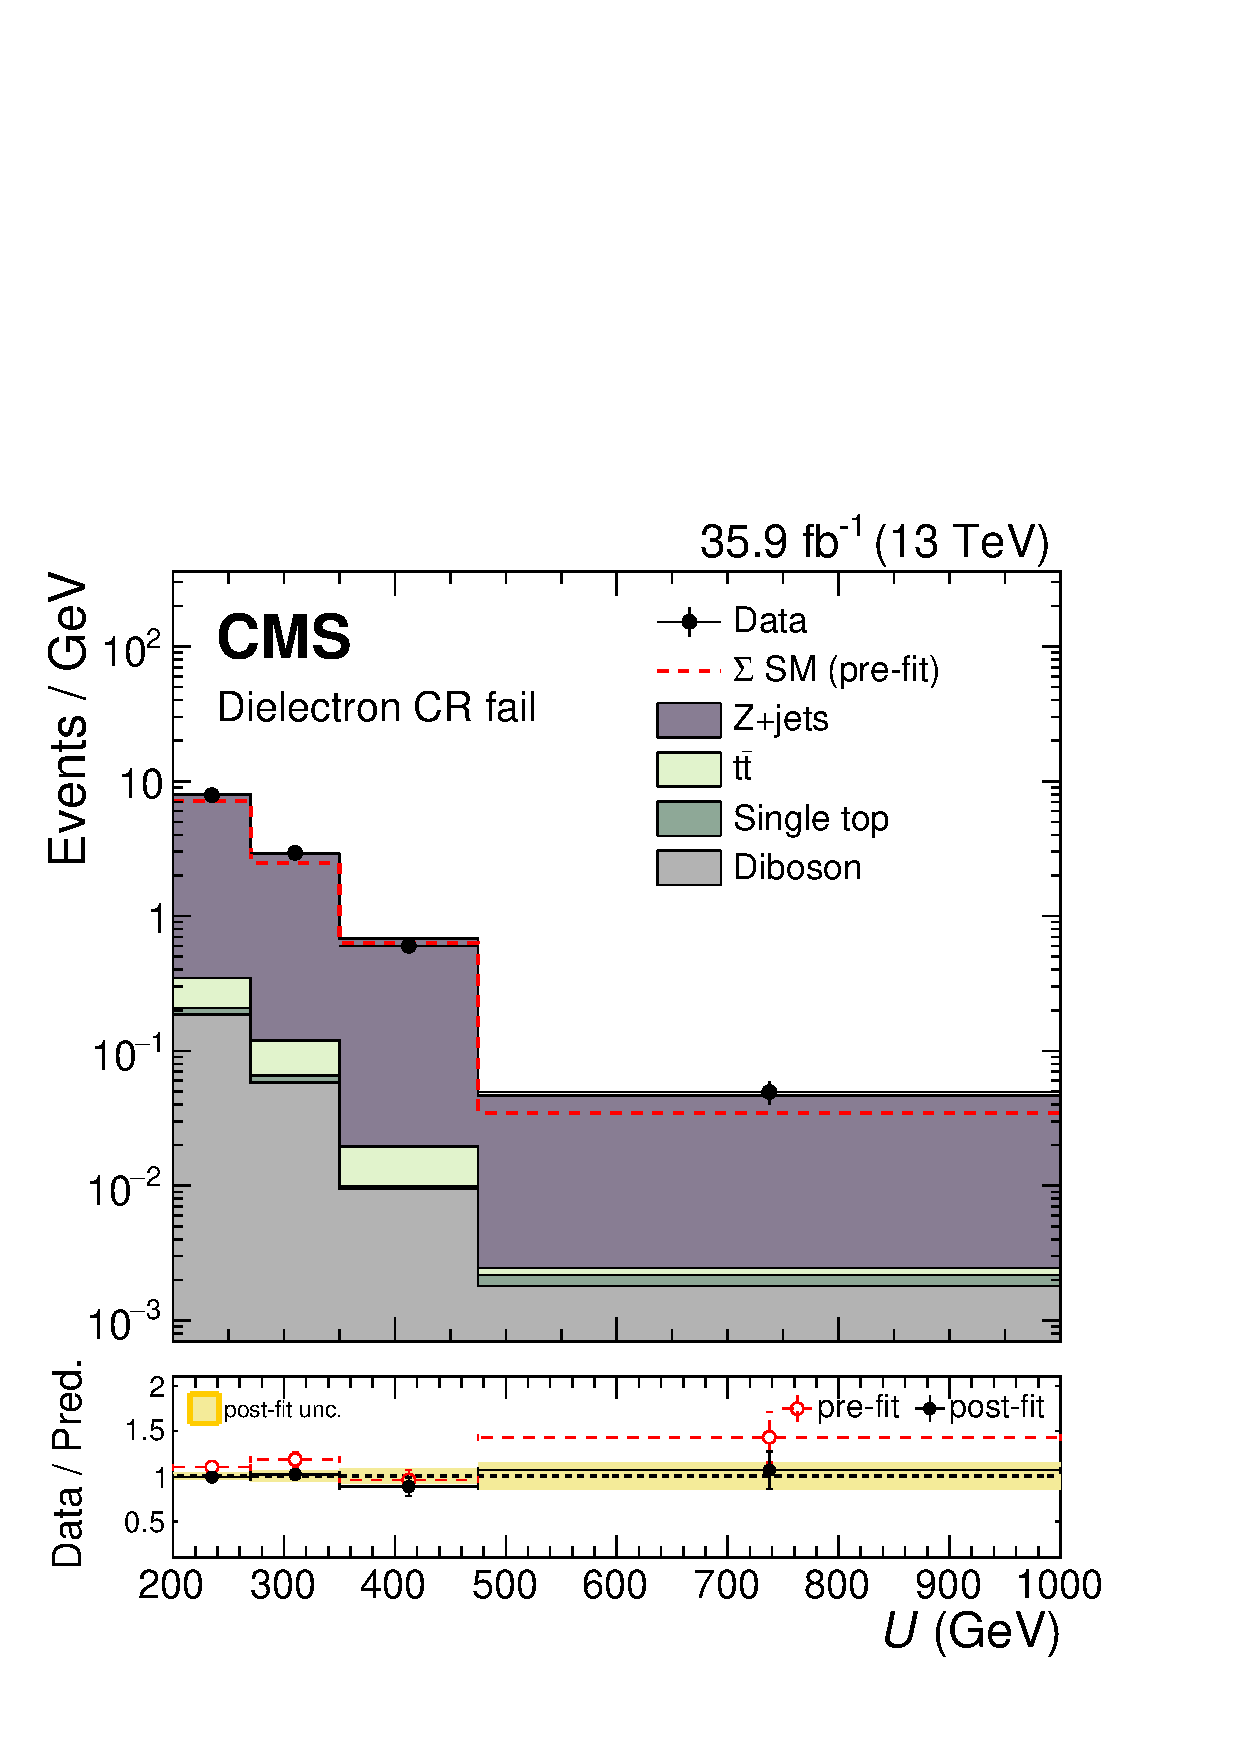
\includegraphics[width=0.36\textwidth]{figures/dataMC/MSDcorr_stackedPostfit_dielectron_fail.pdf}} \\
 \subfloat{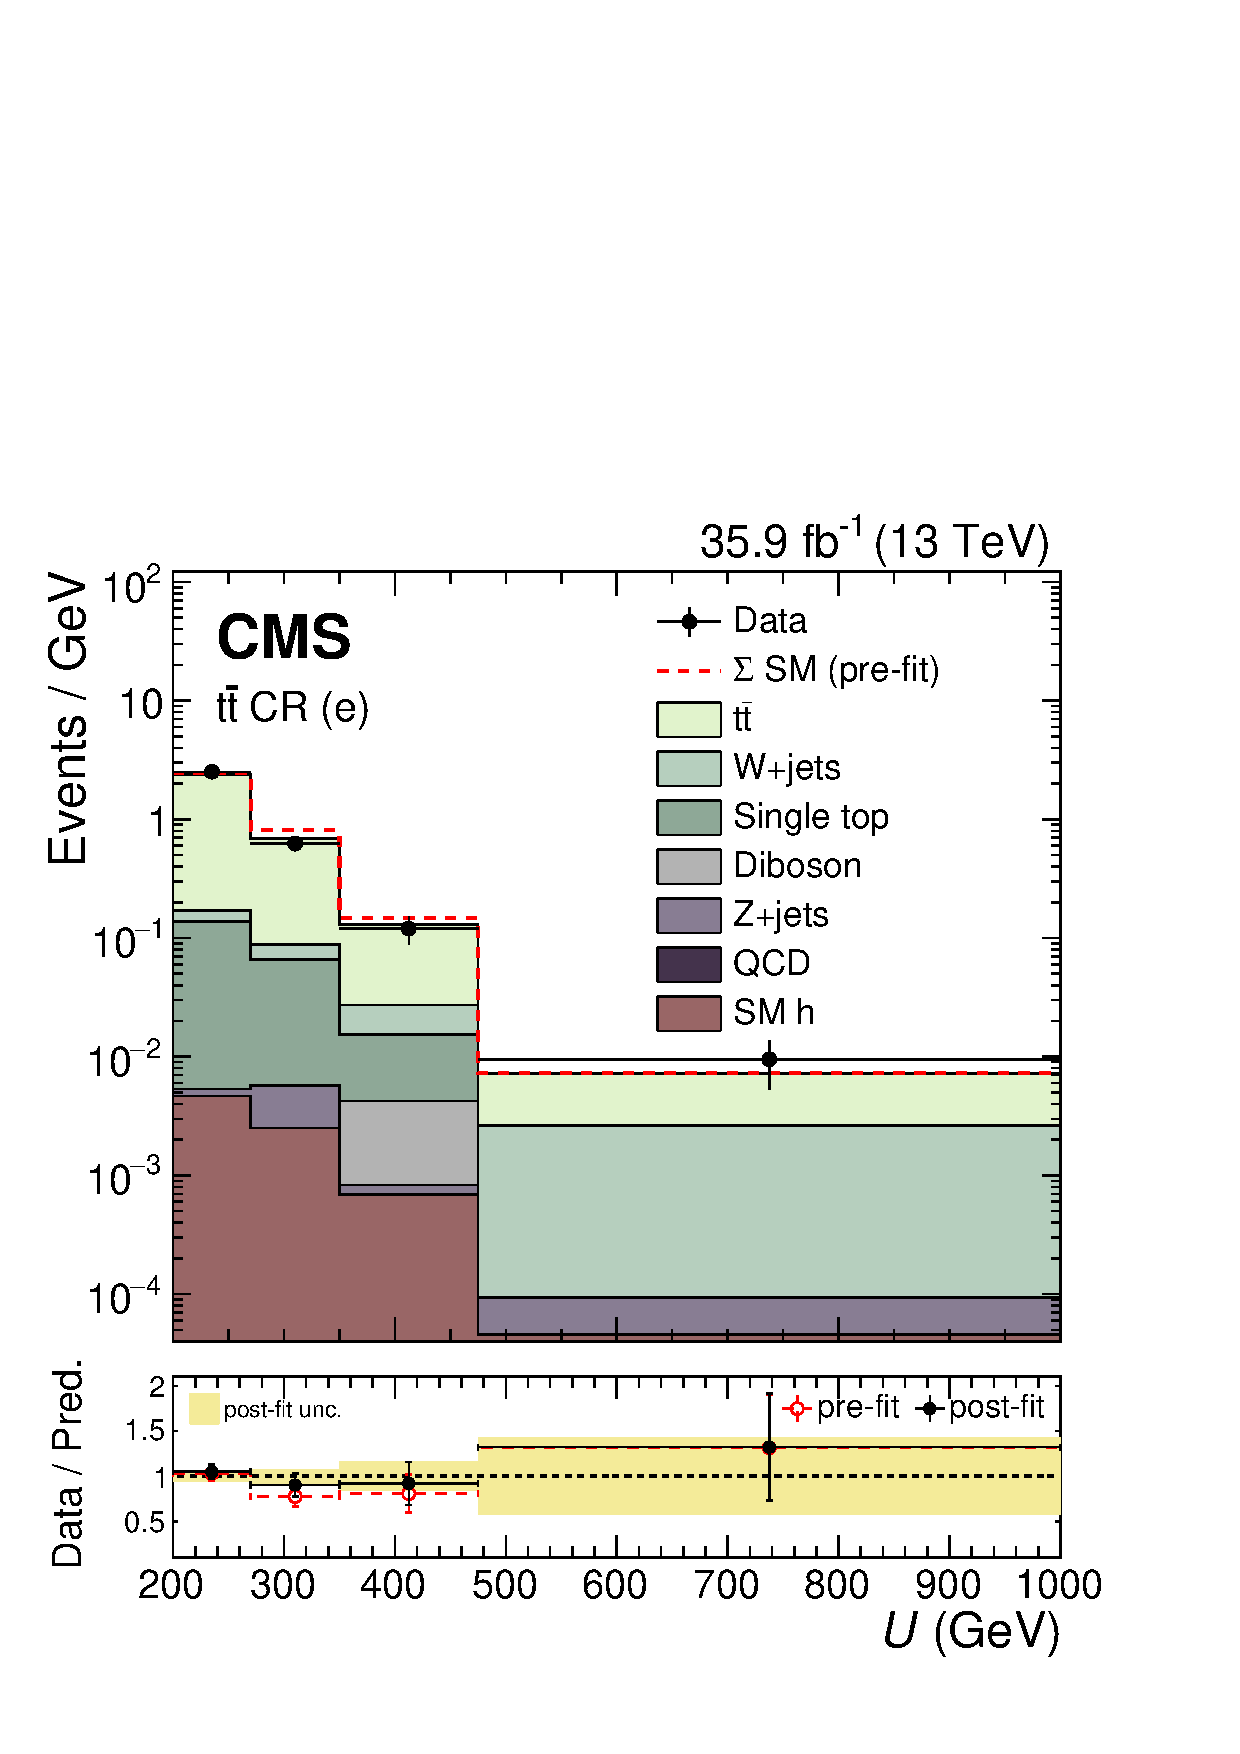
\includegraphics[width=0.36\textwidth]{figures/dataMC/MSDcorr_stackedPostfit_singleelectrontop.pdf}}
 \subfloat{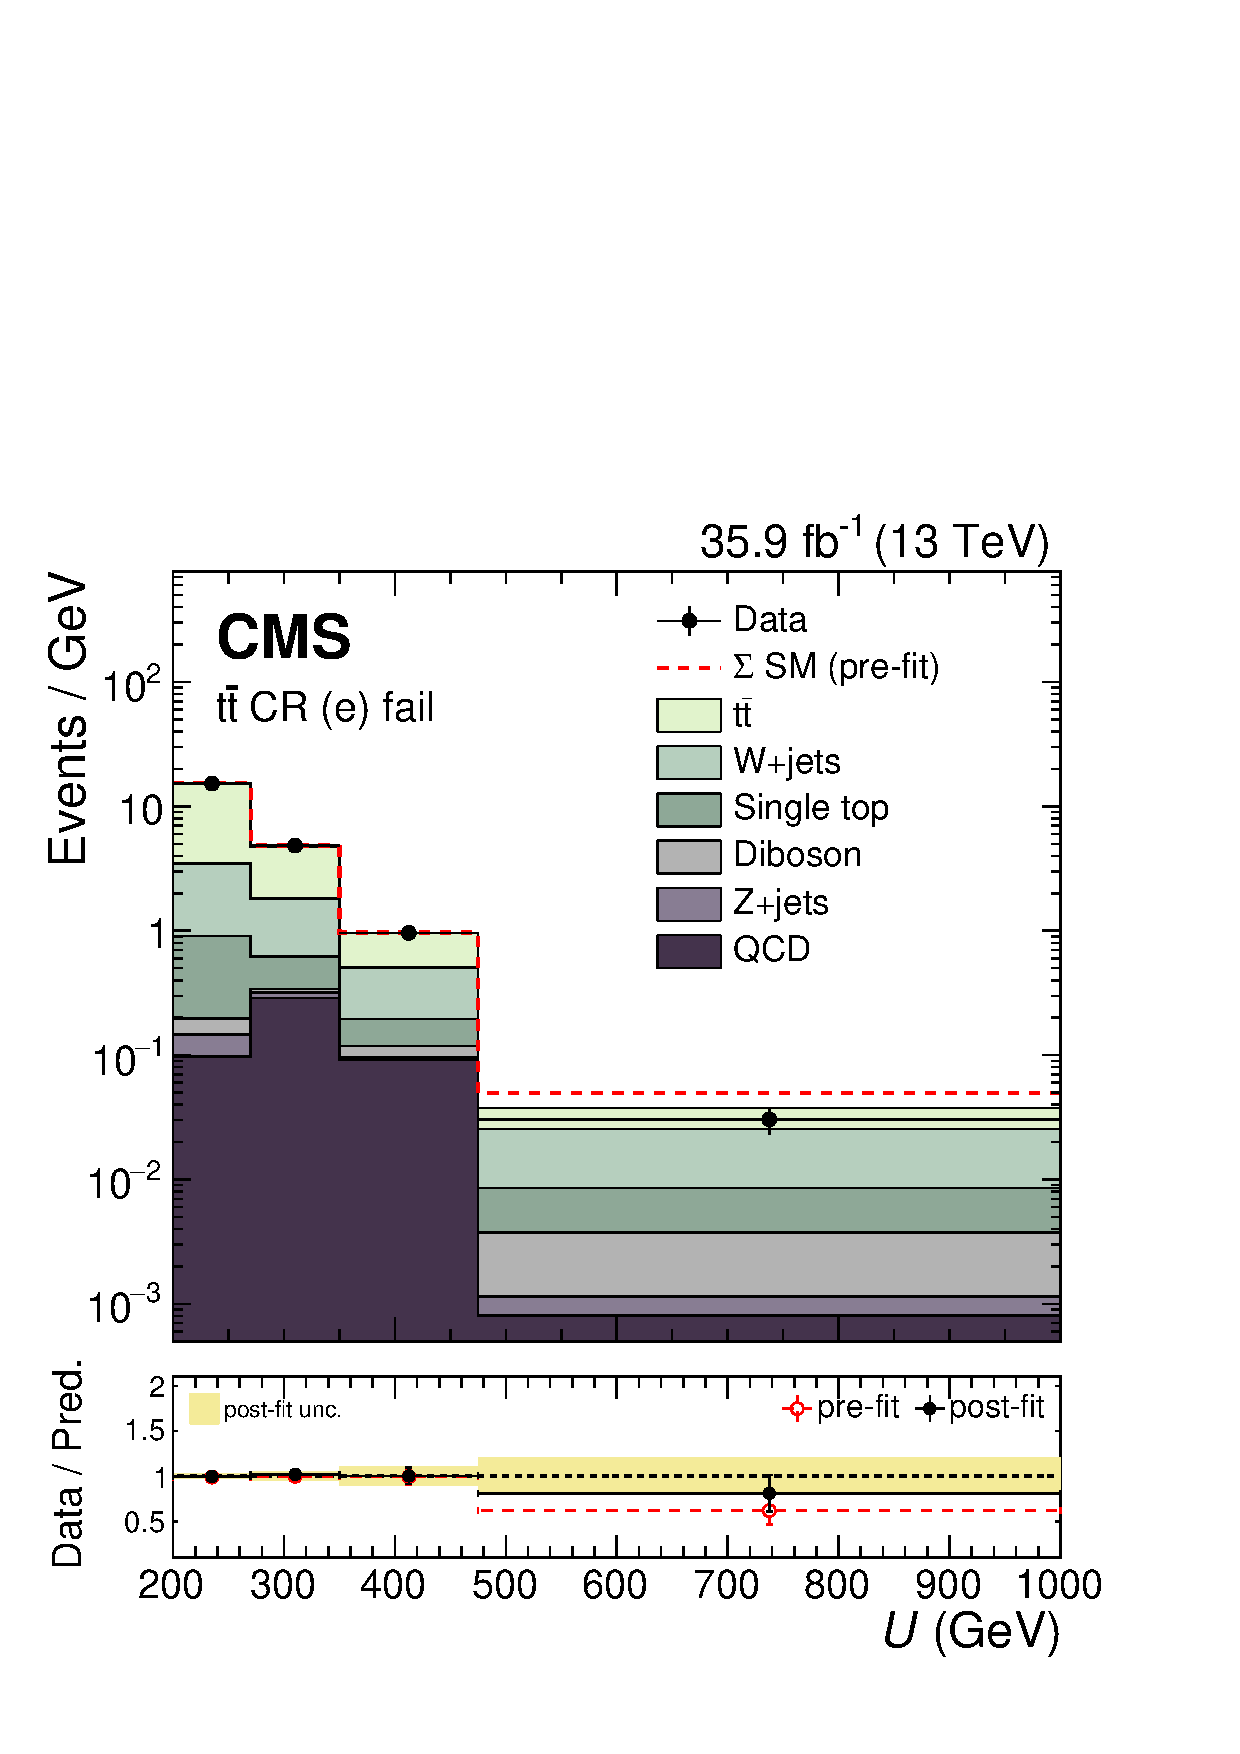
\includegraphics[width=0.36\textwidth]{figures/dataMC/MSDcorr_stackedPostfit_singleelectrontop_fail.pdf}} \\
 \subfloat{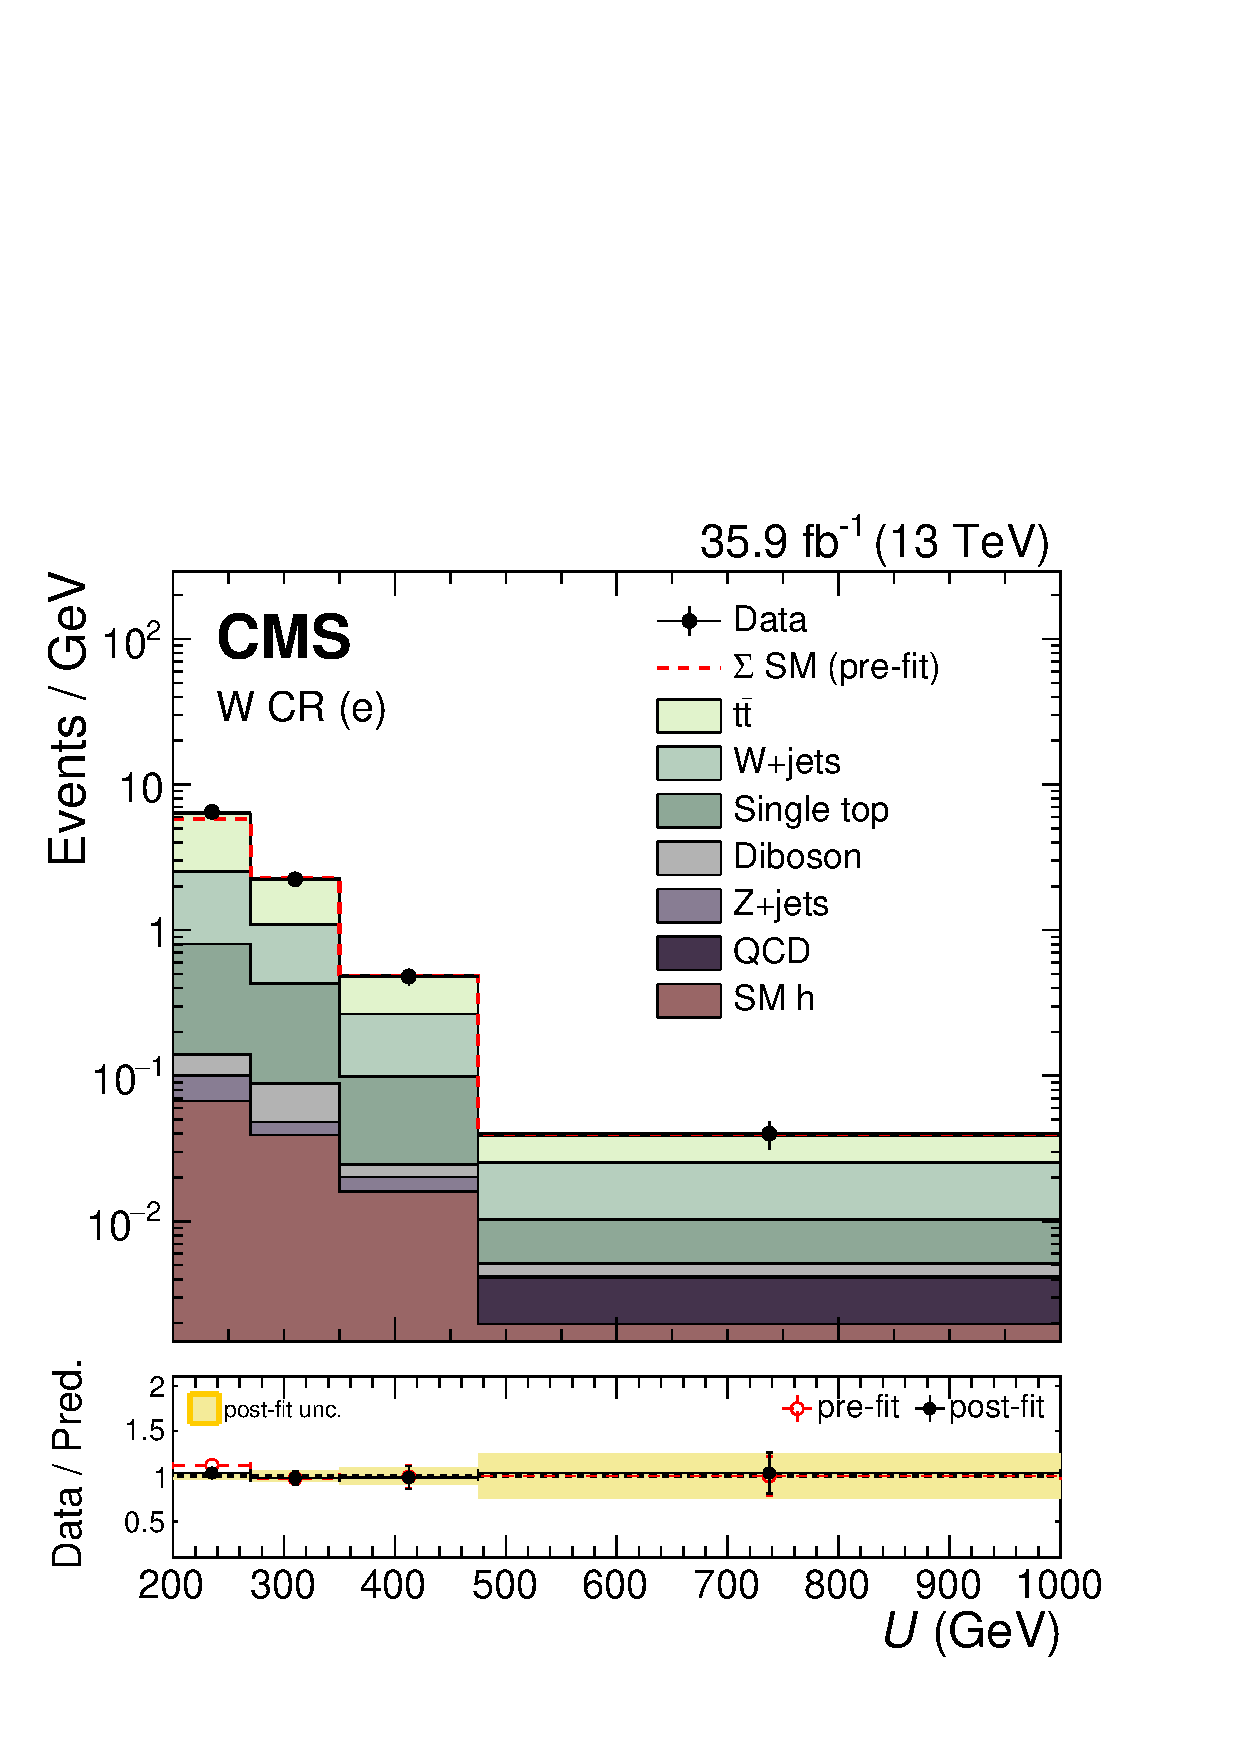
\includegraphics[width=0.36\textwidth]{figures/dataMC/MSDcorr_stackedPostfit_singleelectronw.pdf}}
 \subfloat{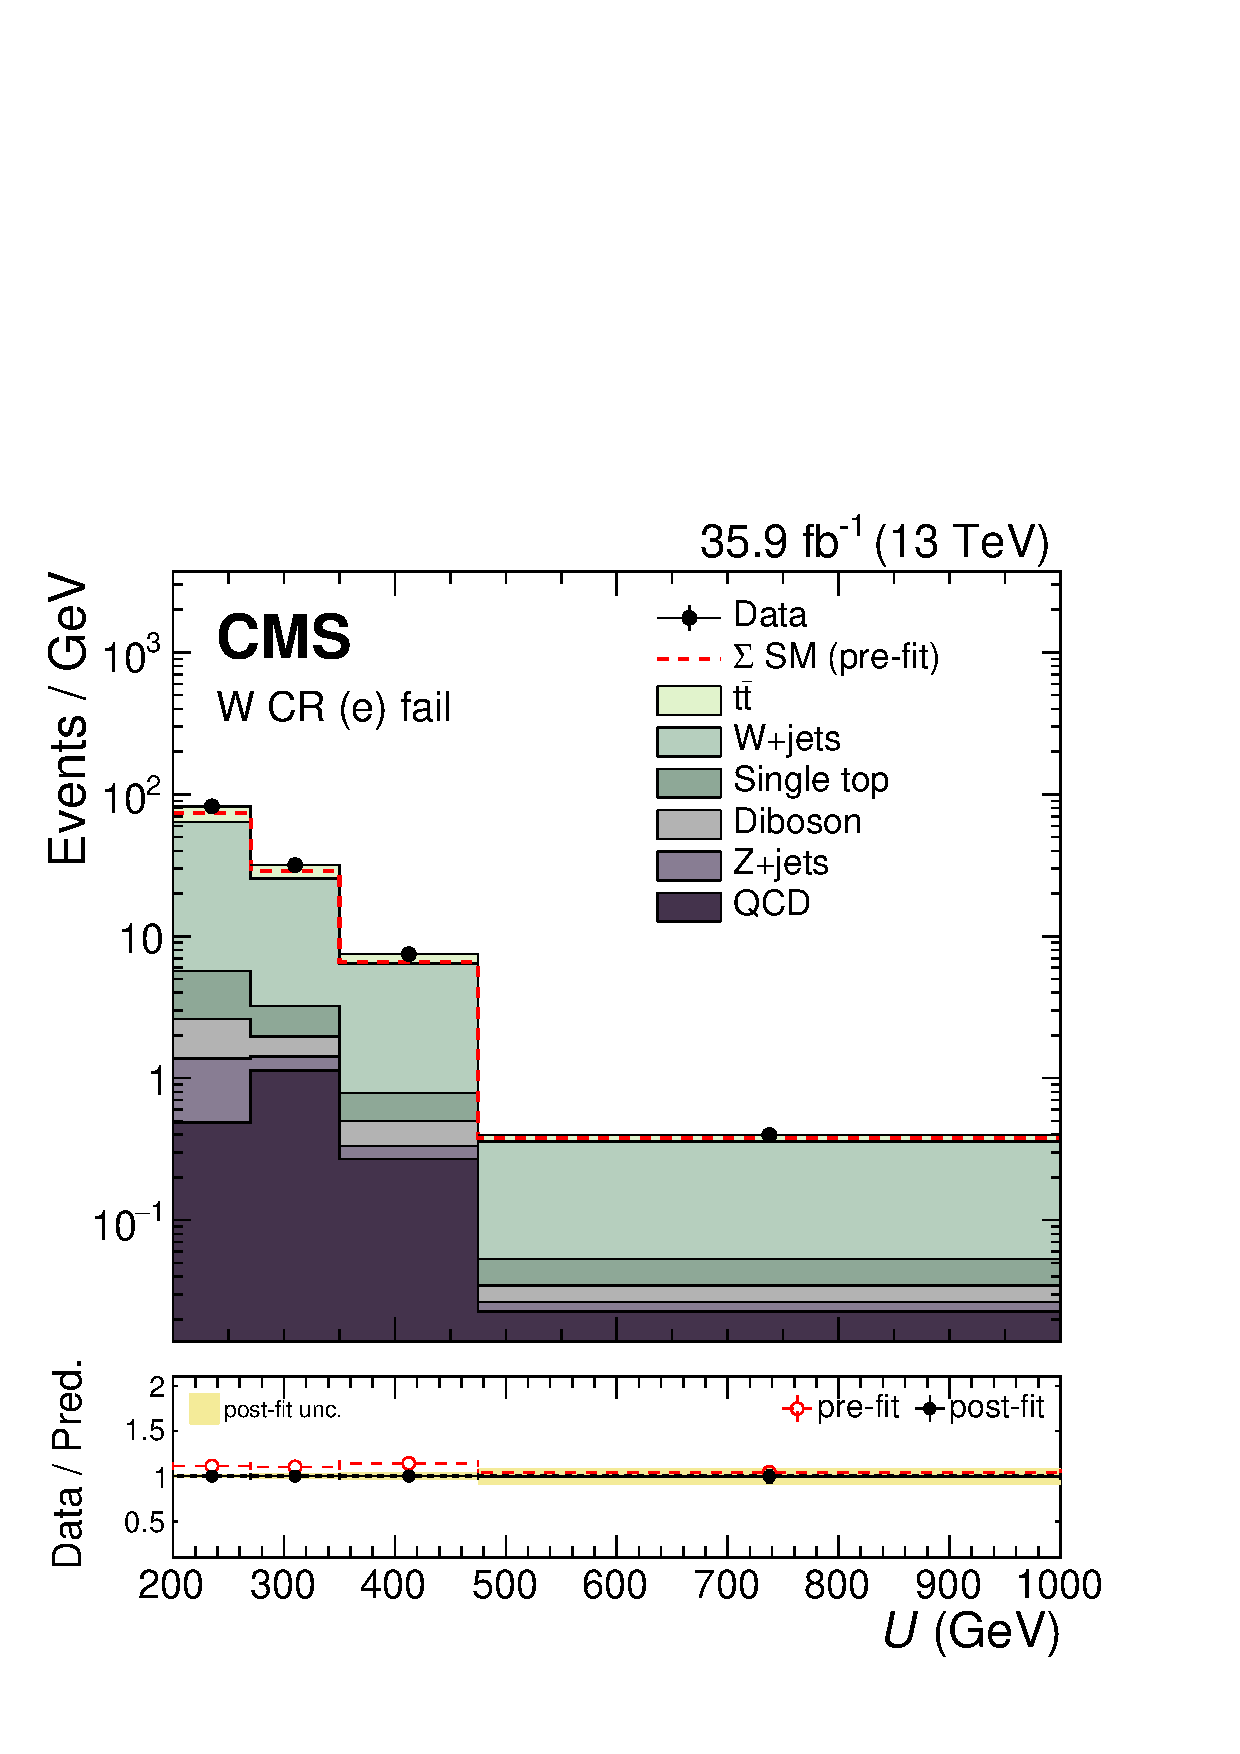
\includegraphics[width=0.36\textwidth]{figures/dataMC/MSDcorr_stackedPostfit_singleelectronw_fail.pdf}} \\
\caption{The $U$ distribution in the electron control regions after a fit to data, including the data in the signal region in the likelihood. Samples in the left distributions are selected with a passing requirement on the double-b tagger; a failing requirement is applied in the distributions to the right.}
\label{Fig_cr_2}
\end{figure}

Since no significant excess over the SM background expectation is observed in the SR, the results of this search are interpreted in terms of upper limits on the signal strength modifier $\mu=\sigma/\sigma_\text{theory}$, where $\sigma_\text{theory}$ is the predicted production cross 
section of DM candidates in association with a Higgs boson and $\sigma$ the upper limit on the observed cross section. 
The upper limits are calculated at 95\% confidence level (CL) using a modified frequentist method (CL$_s$) \cite{yellowReport, bib:CLS1, bib:CLS2} computed with an asymptotic approximation \cite{bib:CLS3}. 


\begin{table}\footnotesize
\begin{center}
  \caption{Per-\ptmiss-bin post-fit event yield expectations for the SM backgrounds in the signal region when including the signal region data in the likelihood fit. Quoted are also pre-fit yields for two signal models. For the 2HDM+a model, we choose $\sin\theta=0.35$ and $\tan\beta=1$. Uncertainties quoted on the predictions include systematic and statistical uncertainties.}
\begin{tabular}{l r r r r}
  \hline\hline
\ptmiss-bin         & 200-270\,GeV          & 270-350\,GeV          & 350-475\,GeV          & $>475$\,GeV         \\
\hline
Z+jets          &$ 248.9\pm22.2 $       & $97.2\pm8.5$         & $32.6\pm3.6$          & $11.1\pm1.9$       \\
\ttbar          &$ 199.2\pm13.5 $       & $52.1\pm5.2$          & $11.1\pm2.0$          & $0.7\pm0.4$        \\
W+jets          &$ 121.6\pm21.6 $       & $45.0\pm8.7$          & $8.4\pm1.9$           & $2.9\pm0.9$            \\
Single top      &$21.0\pm4.2 $          & $6.1\pm1.2$           & $0.9\pm0.2$           & $0.2\pm0.1$         \\
Diboson         &$ 16.0\pm3.1  $        & $7.6\pm1.5$           & $2.4\pm0.5$           & $1.0\pm0.2$ \\
SM h             &$ 12.6\pm1.4 $      & $ 6.6\pm0.7$           & $ 3.3 \pm 0.3$        & $ 1.3\pm 0.1$      \\
\hline
$\Sigma~(\text{SM})$ & $619.3\pm20.1$ & $214.6 \pm 8.1$       & $58.7\pm3.7$          & $17.2 \pm 2.0$ \\
\hline
2HDM+a, $m_\text{A}=1\TeV$, $m_\text{a}=150$\GeV & $5.7 \pm 0.6$ & $9.8 \pm 1.1$ & $18.5 \pm 2.1$ & $5.2 \pm 0.6$\\
Bar. Z', $m_{\text{Z}'}=0.2\TeV$, $m_\chi=50$\GeV & $184.2 \pm 20.0$ & $118.1 \pm 12.8$ & $69.5 \pm 7.7$ & $28.9 \pm 3.3$\\

\hline
Data            & $619$       & $ 214$        & $59$          & $ 21$ \\
\hline\hline
  \end{tabular}
\label{tab:eventYieldTable}
\end{center}
\end{table}

\begin{table}\footnotesize
\begin{center}
  \caption{Per-\ptmiss-bin post-fit event yield expectations for the SM backgrounds in the signal region when masking the signal region data from the likelihood fit. Uncertainties quoted on the predictions include systematic and statistical uncertainties.}
\begin{tabular}{l r r r r}
  \hline\hline
\ptmiss-bin         & 200-270\,GeV          & 270-350\,GeV          & 350-475\,GeV          & $>475$\,GeV         \\
\hline
Z+jets          &$ 239.2\pm37.9 $       & $93.3\pm14.4$         & $31.1\pm5.5$          & $10.0\pm2.2$       \\
\ttbar          &$ 200.0\pm13.3 $       & $52.3\pm5.1$          & $11.1\pm2.0$          & $0.7\pm0.4$        \\
W+jets          &$ 119.8\pm22.4 $       & $44.3\pm8.9$          & $8.3\pm1.9$           & $2.8\pm0.9$            \\
Single top      &$21.0\pm4.3 $          & $6.1\pm1.3$           & $0.9\pm0.2$           & $0.2\pm0.1$         \\
Diboson         &$ 16.0\pm3.1  $        & $7.6\pm1.5$           & $2.4\pm0.5$           & $1.0\pm0.2$ \\
SM h             &$ 12.6\pm1.4 $      & $ 6.6\pm0.7$           & $ 3.3 \pm 0.3$        & $ 1.3\pm 0.1$      \\
\hline
$\Sigma~(\text{SM})$ & $608.3\pm41.8$ & $210.2 \pm 15.9$       & $57.1\pm5.7$          & $16.0 \pm 2.2$ \\
\hline
Data            & $619$       & $ 214$        & $59$          & $ 21$ \\
\hline\hline
  \end{tabular}
\label{tab:eventYieldTable_masked}
\end{center}
\end{table}


For the 2HDM+a model, $m_\text{A}$ masses are excluded between 500 and 900\GeV for $m_\text{a}=150\GeV$, $\sin\theta=0.35$ and $\tan\beta=1$. Mixing angles of $0.35<\sin\theta<0.75$ are excluded for $m_\text{A}=600\GeV$ and $m_\text{a}=200\GeV$, assuming $\tan\beta=1$. We can furthermore exclude $\tan\beta$ values between 0.5 and 2.0 (1.6) for $m_\text{a}=100$ (150)\GeV and $m_\text{A}=600\GeV$, given $\sin\theta=0.35$. Figure~\ref{fig:limits_2hdma} shows the upper limits on $\mu$ for the three scans (mass, $\sin\theta$, and $\tan\beta$) performed.


\begin{figure}[htbp]
  \centering
  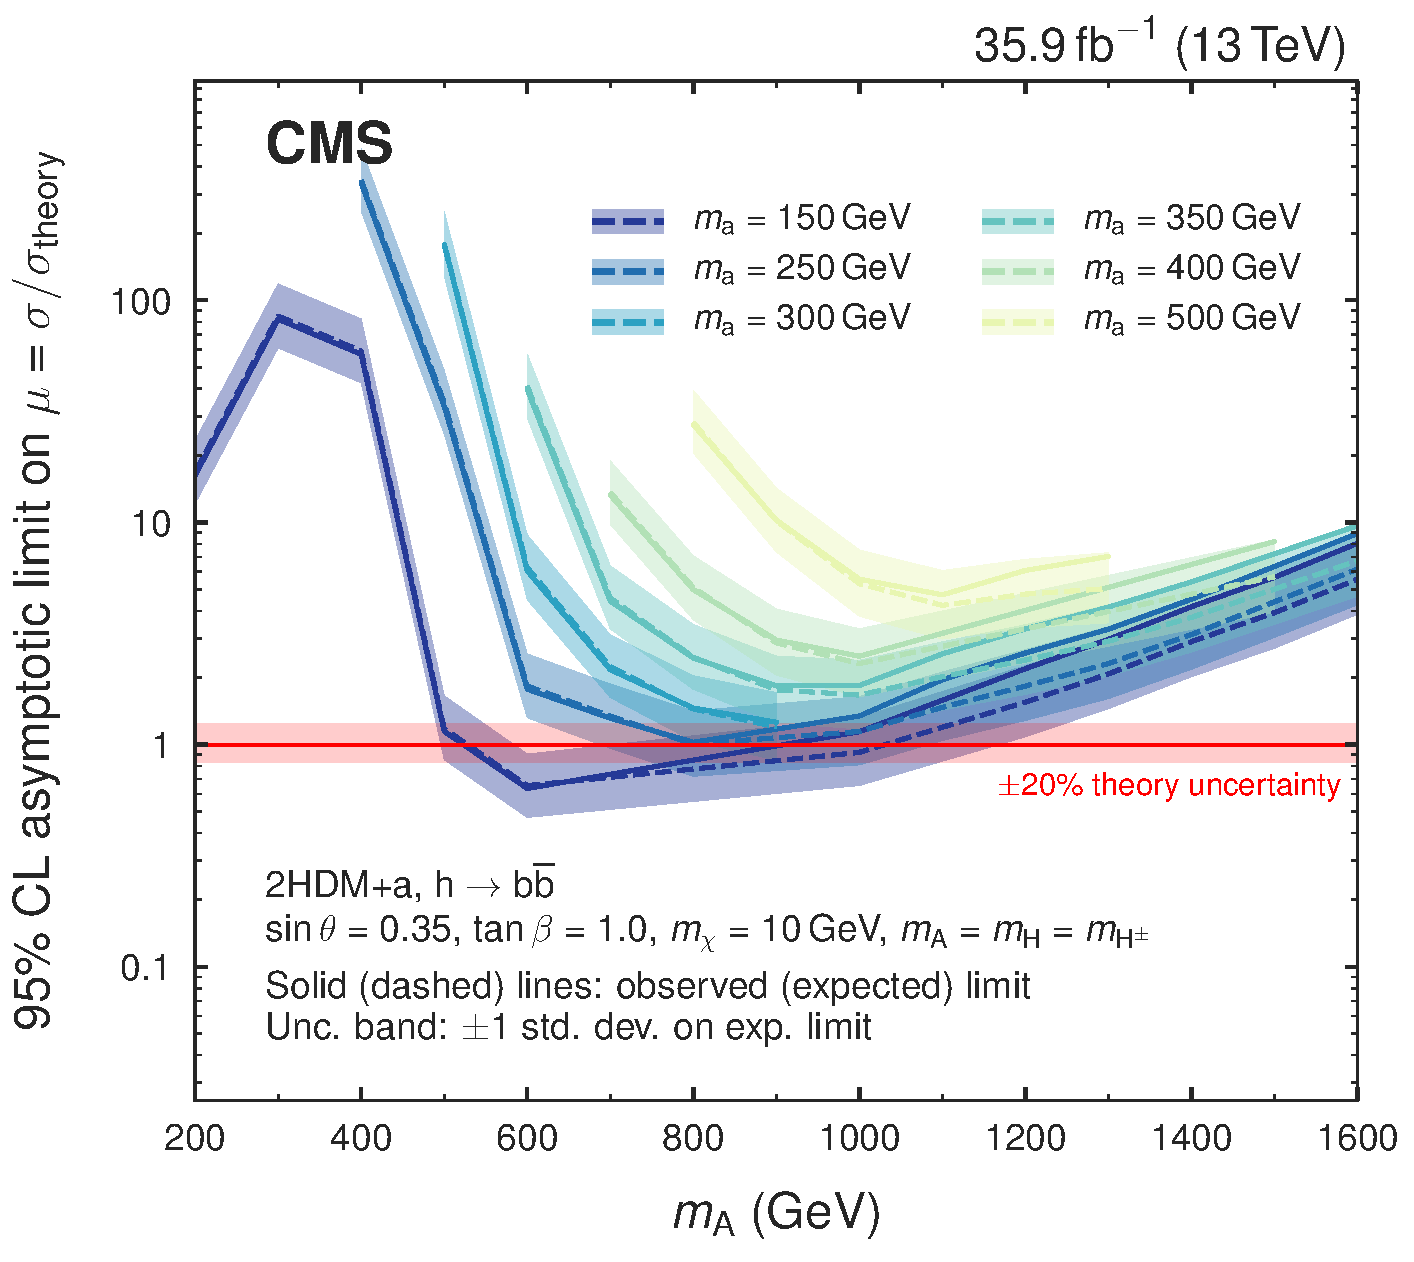
\includegraphics[width=0.475\textwidth]{figures/limits/limits_2hdma_mass.pdf}
  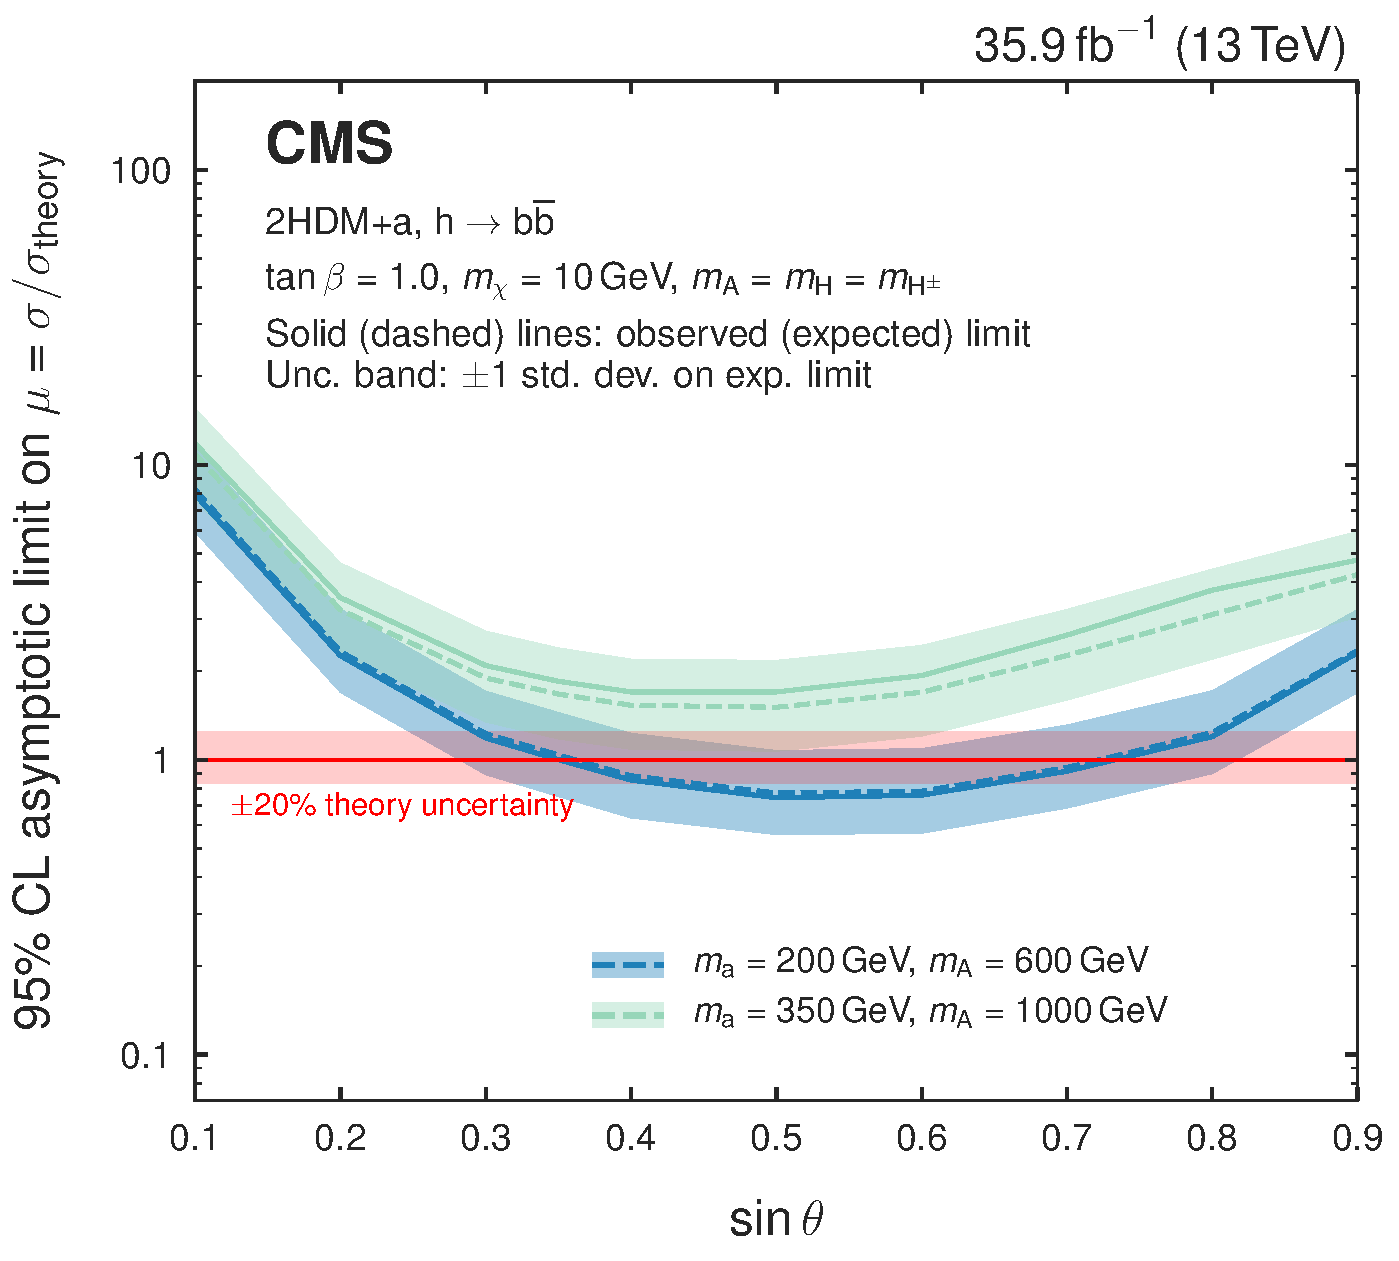
\includegraphics[width=0.475\textwidth]{figures/limits/limits_2hdma_sinp.pdf}\\
  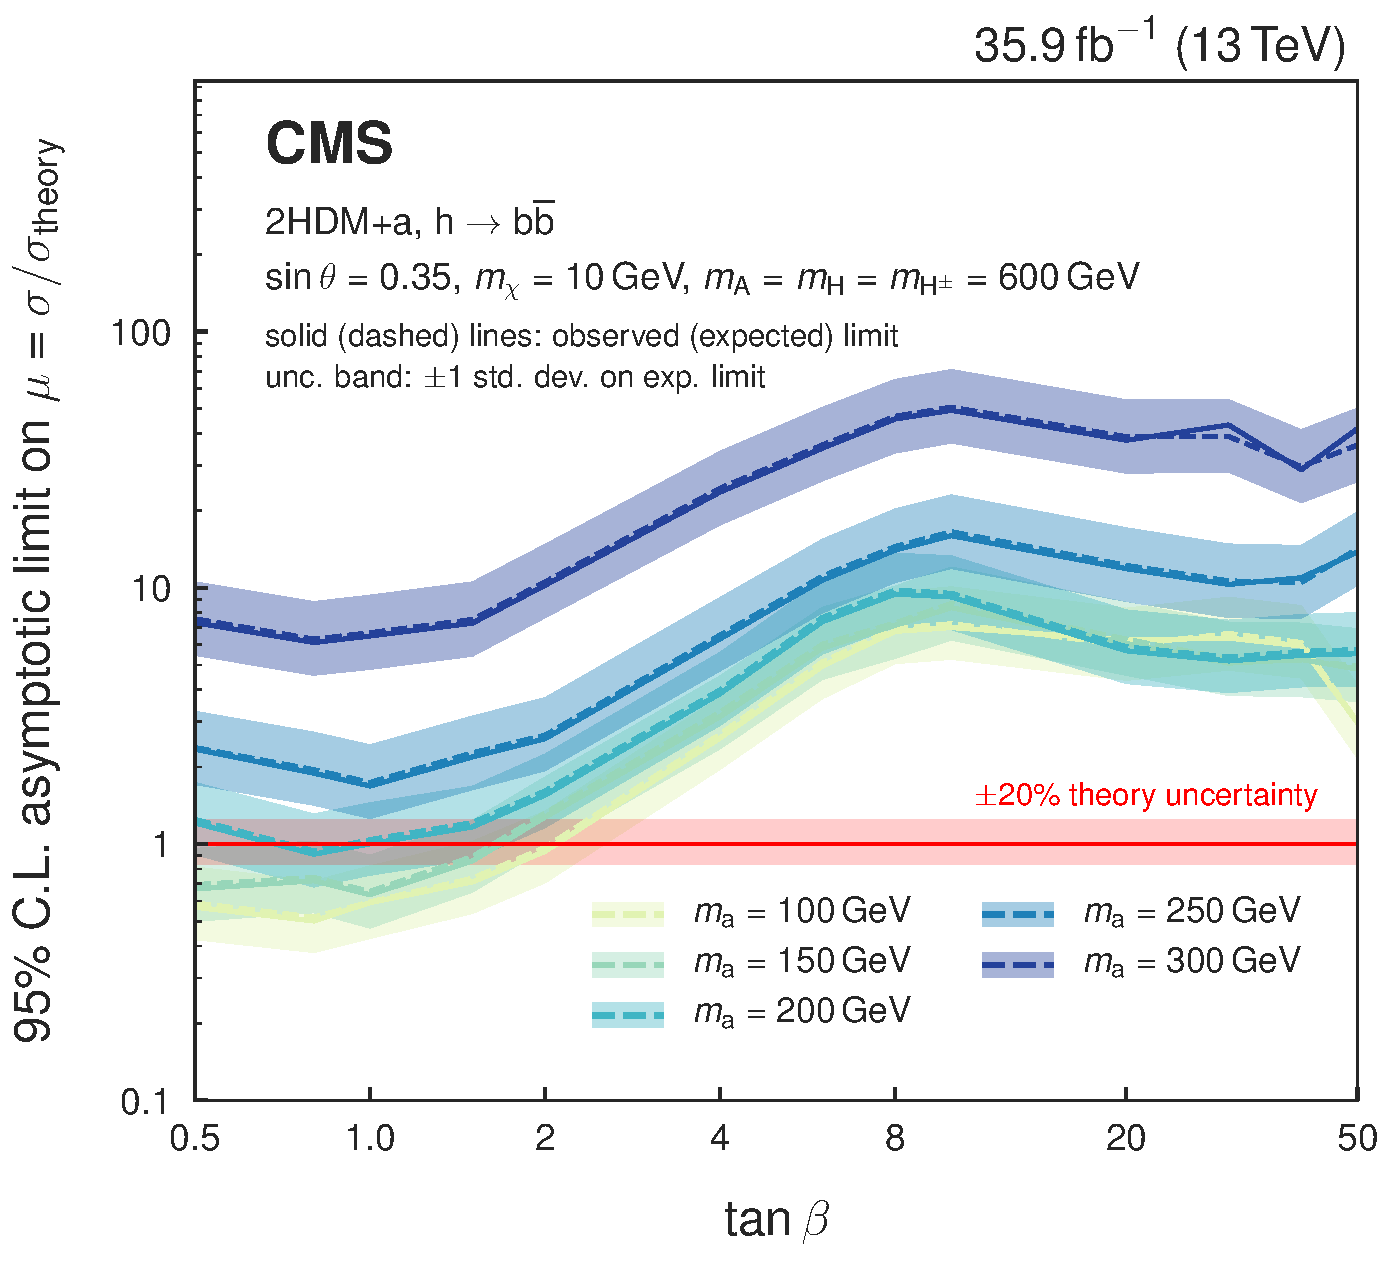
\includegraphics[width=0.475\textwidth]{figures/limits/limits_2hdma_tanb.pdf}\\
  \caption{Upper limits on the signal strength modifier for the 2HDM+a model when scanning in the $m_\text{A}$-$m_\text{a}$ plane (upper left), the mixing angle $\theta$ (upper right), or $\tan\beta$ (bottom).}
  \label{fig:limits_2hdma}
\end{figure}


\begin{figure}[htbp]
  \centering
%  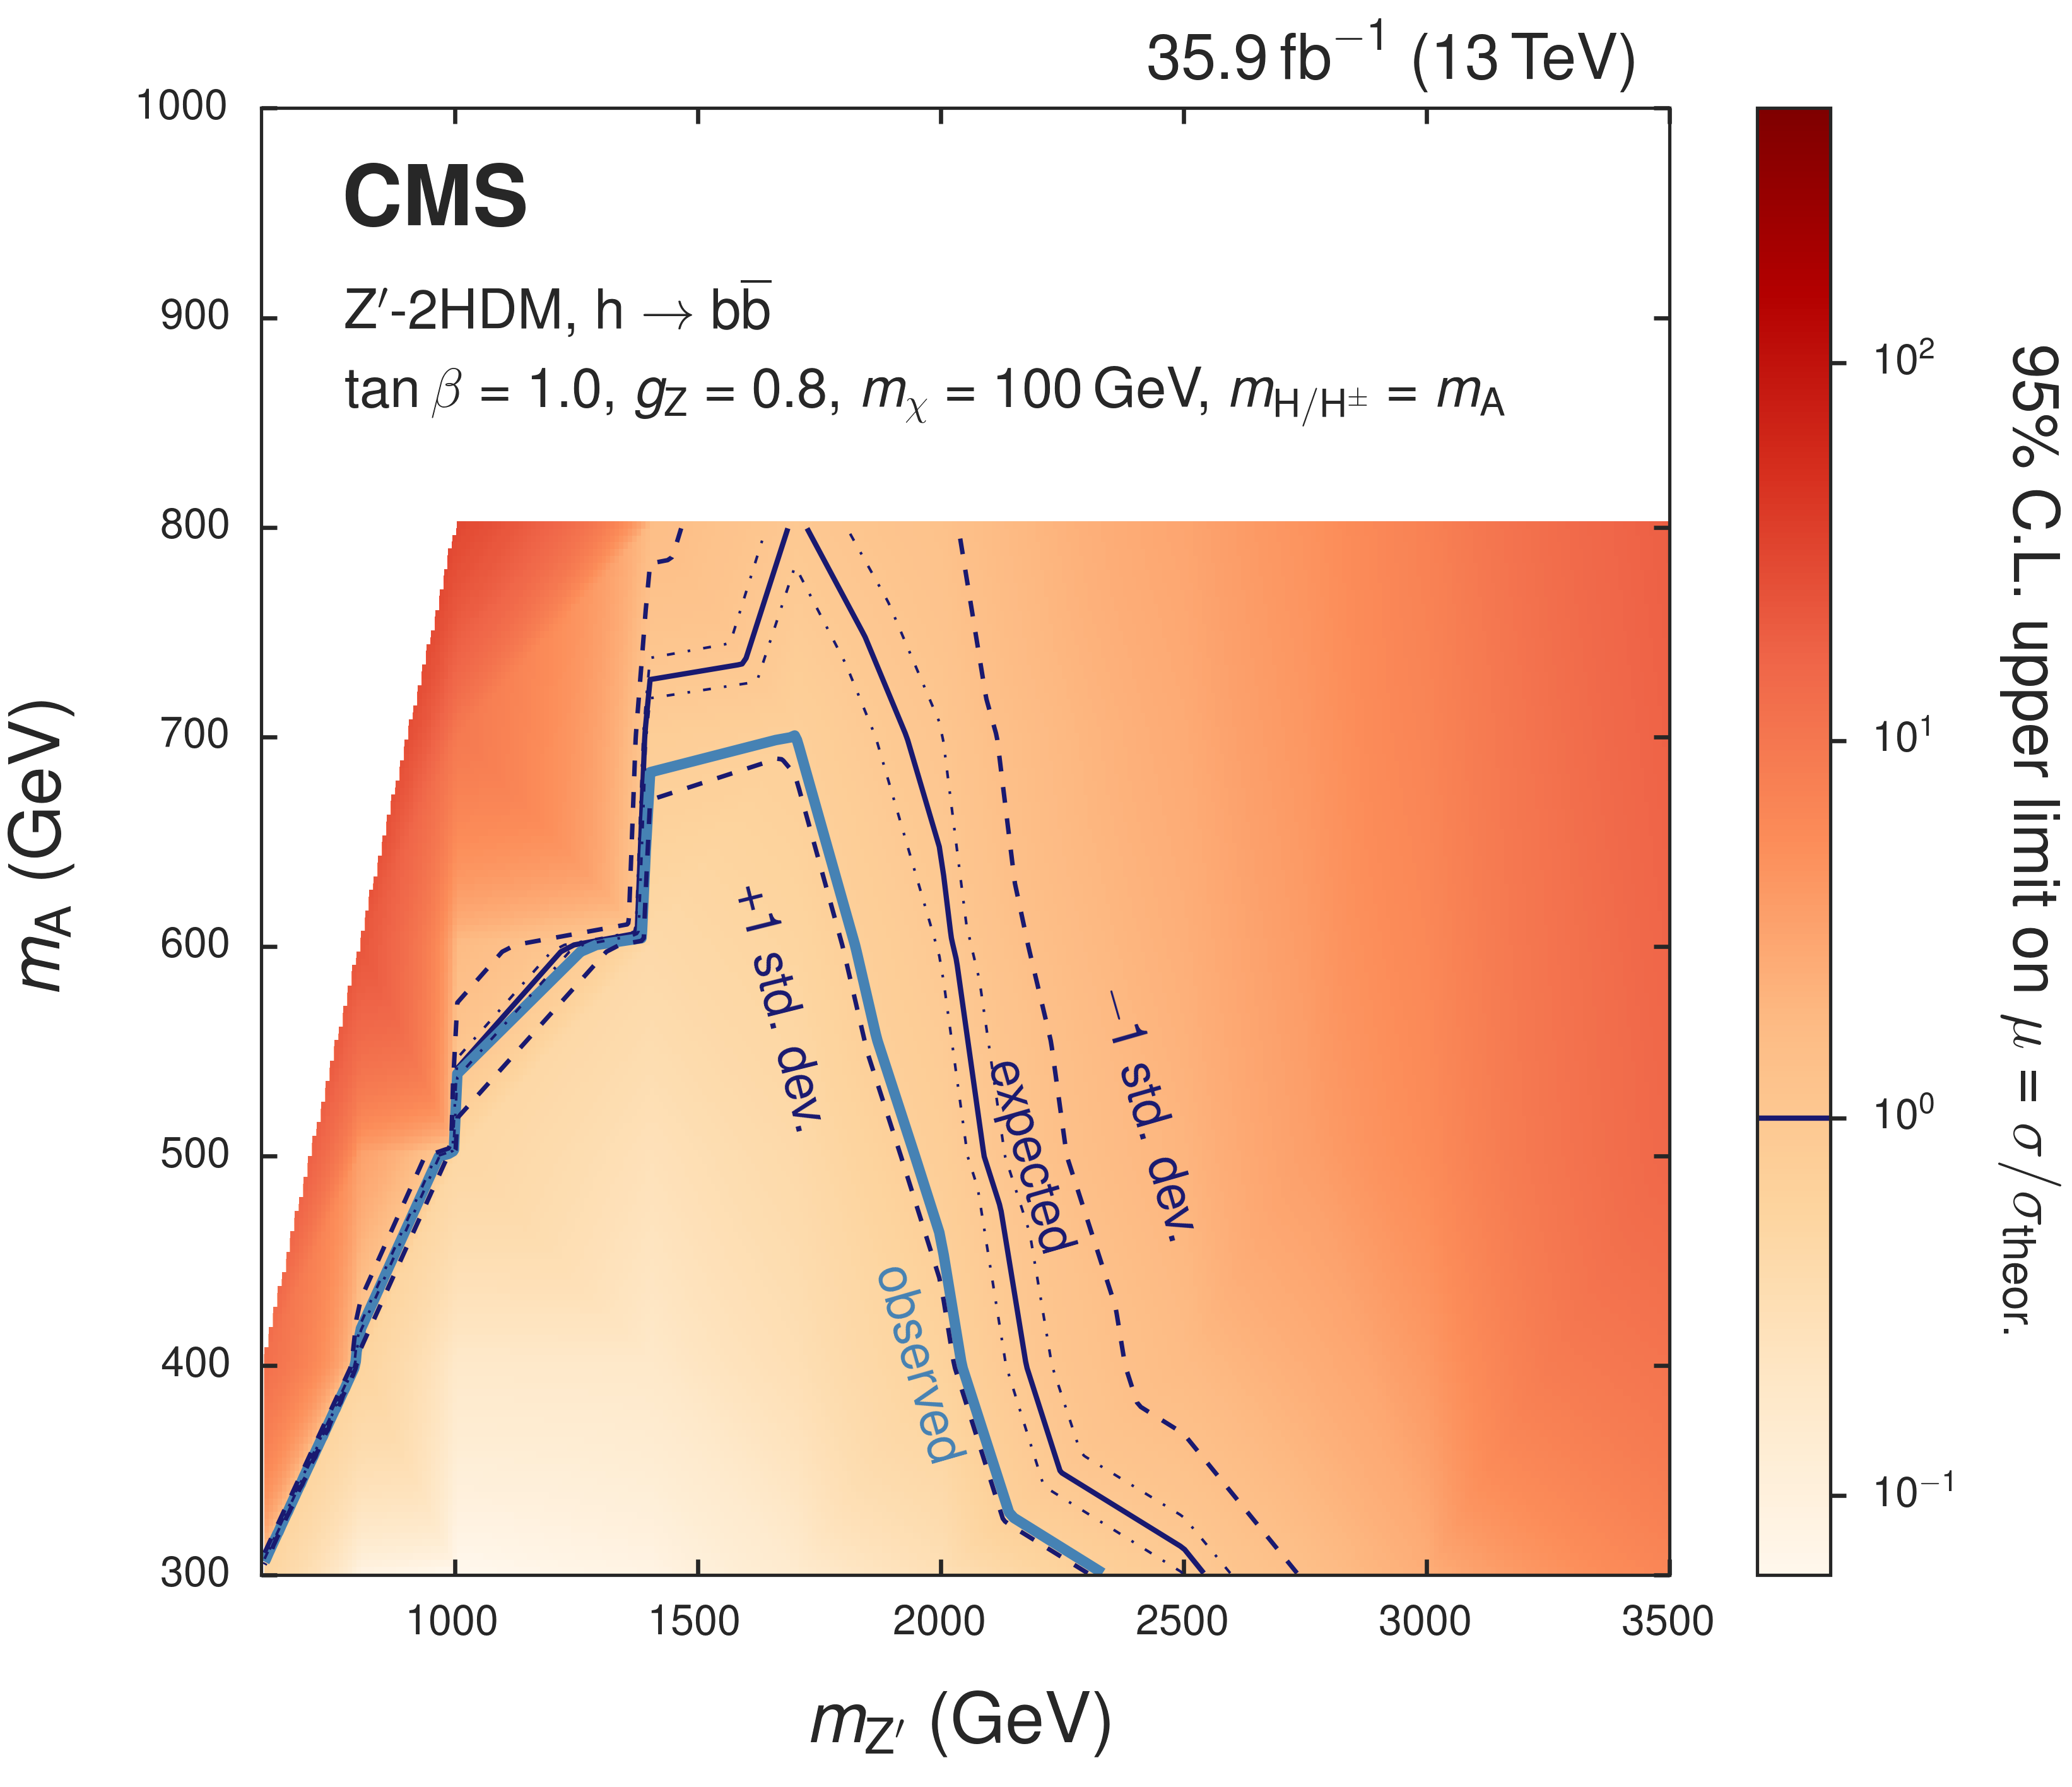
\includegraphics[width=0.475\textwidth]{figures/limits/limits_2hdm2d.png}
%  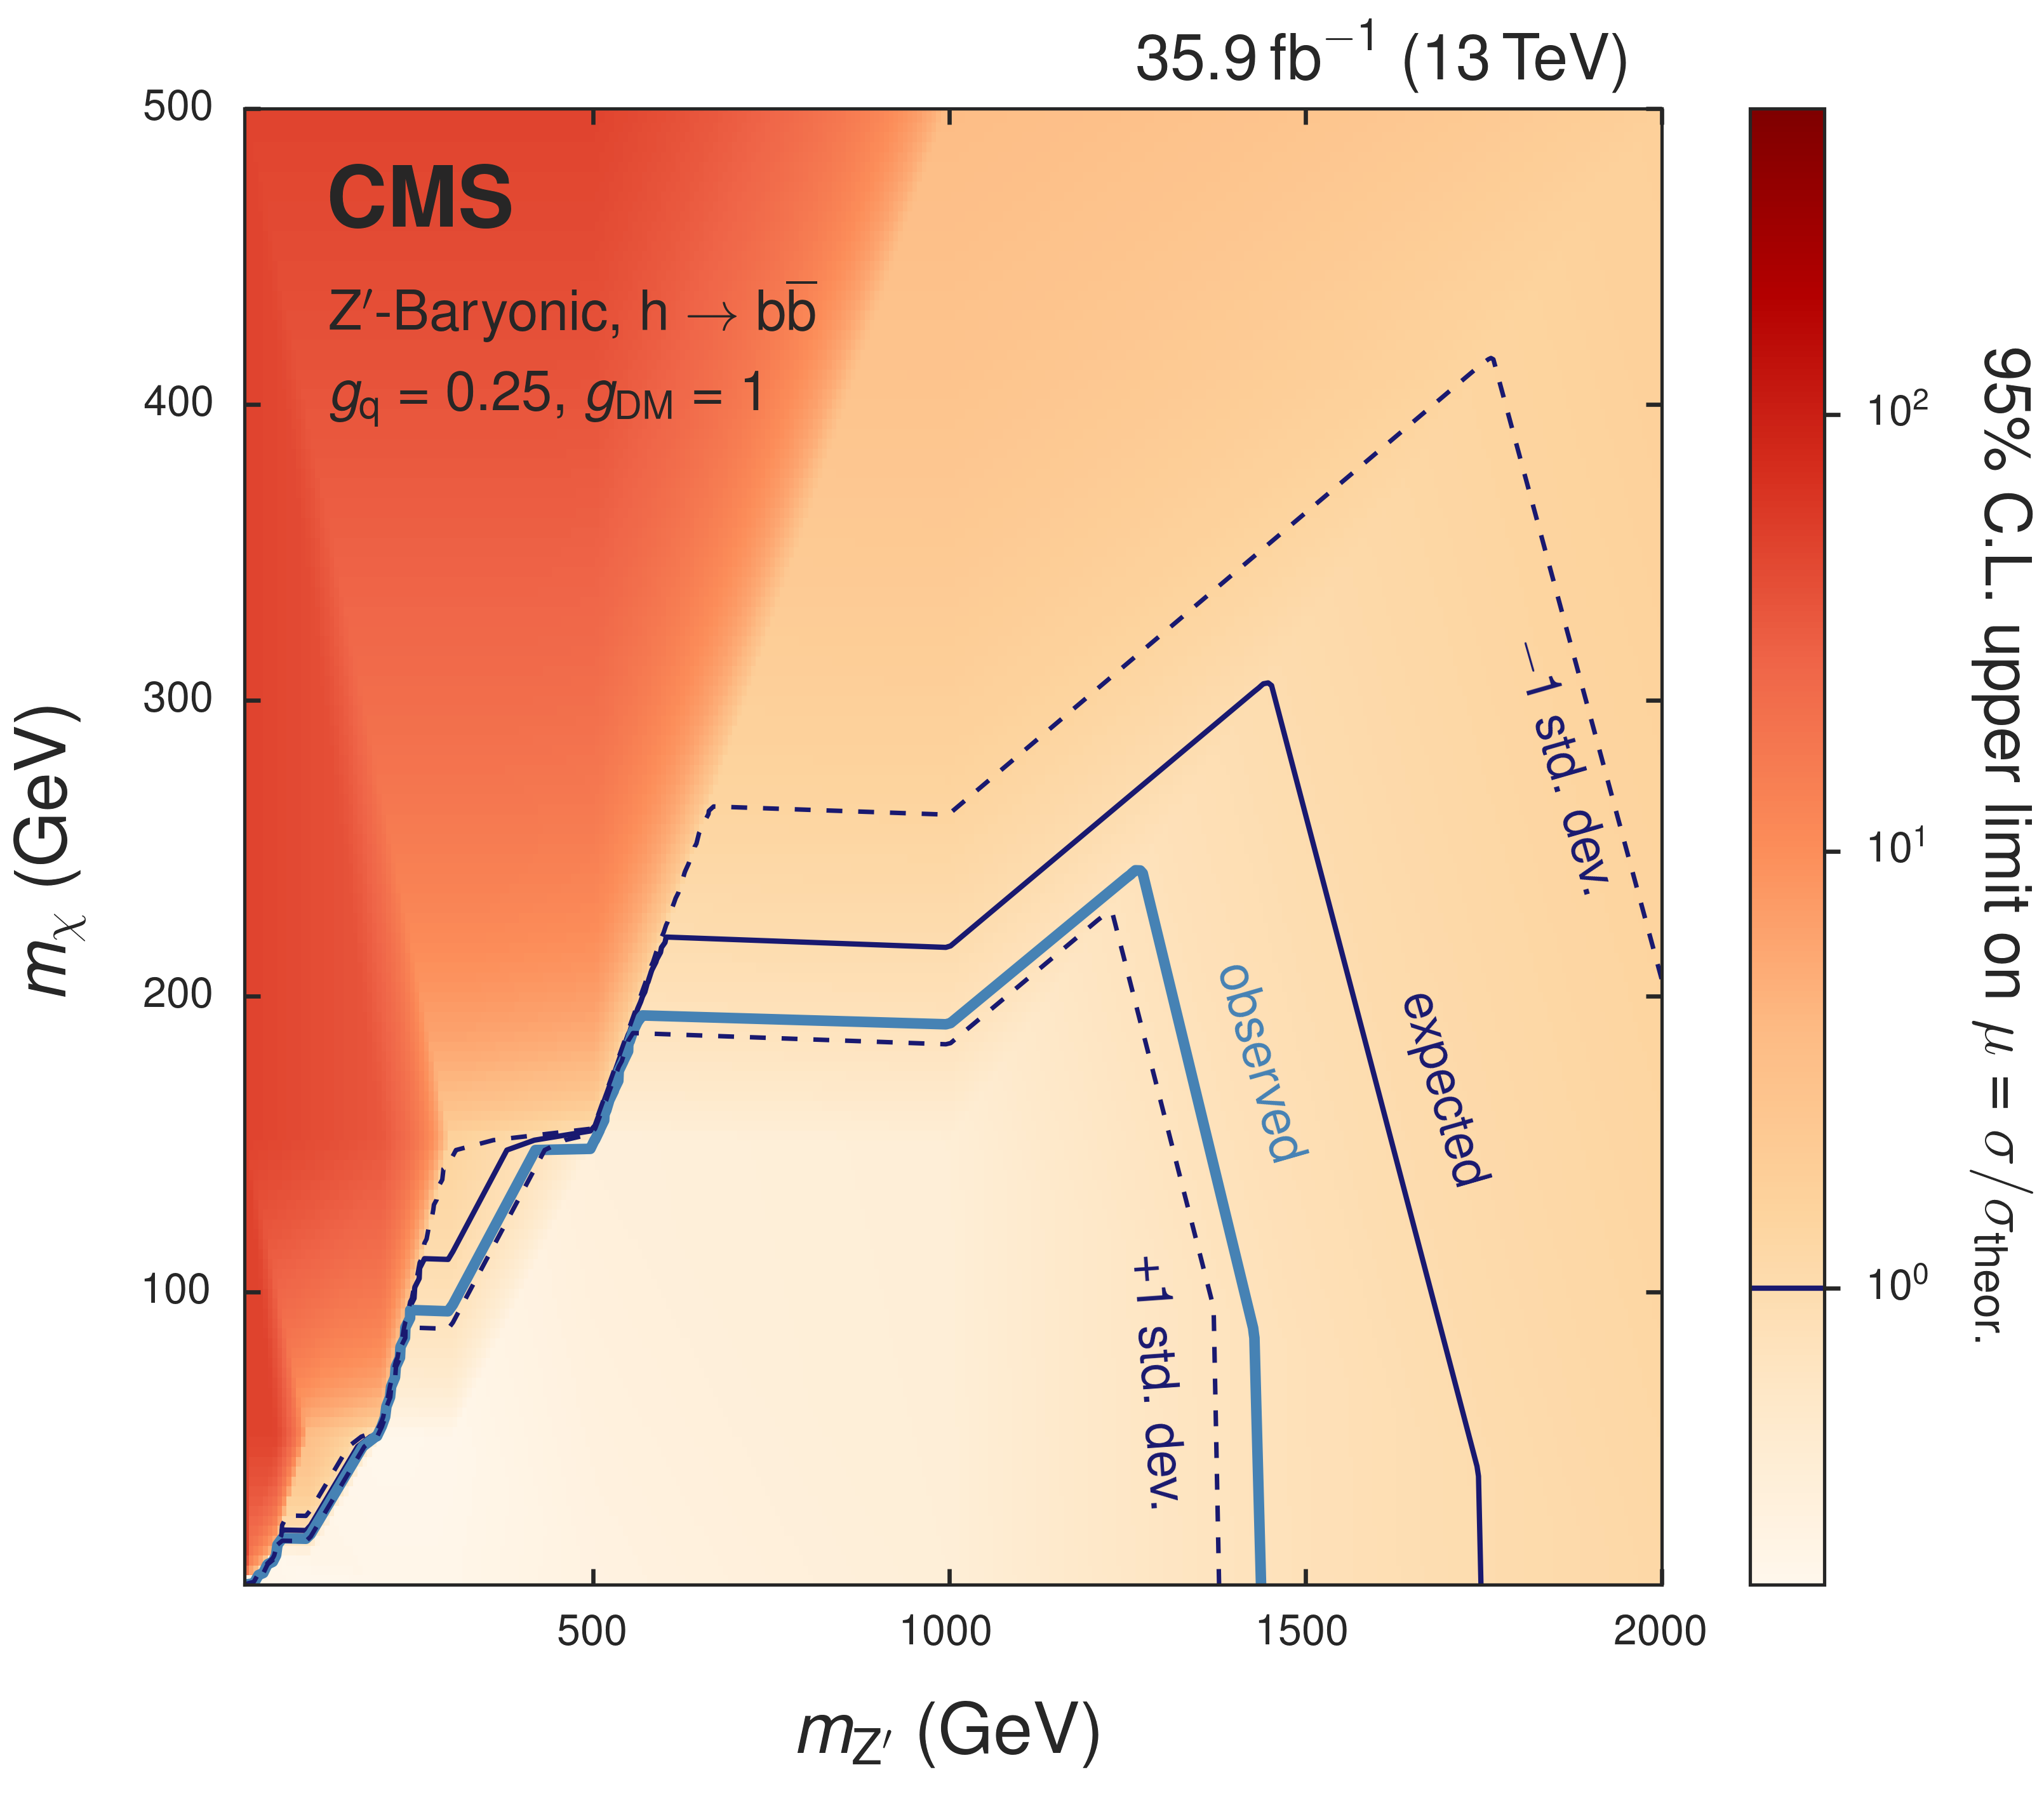
\includegraphics[width=0.475\textwidth]{figures/limits/limits_barzp2d.png}
  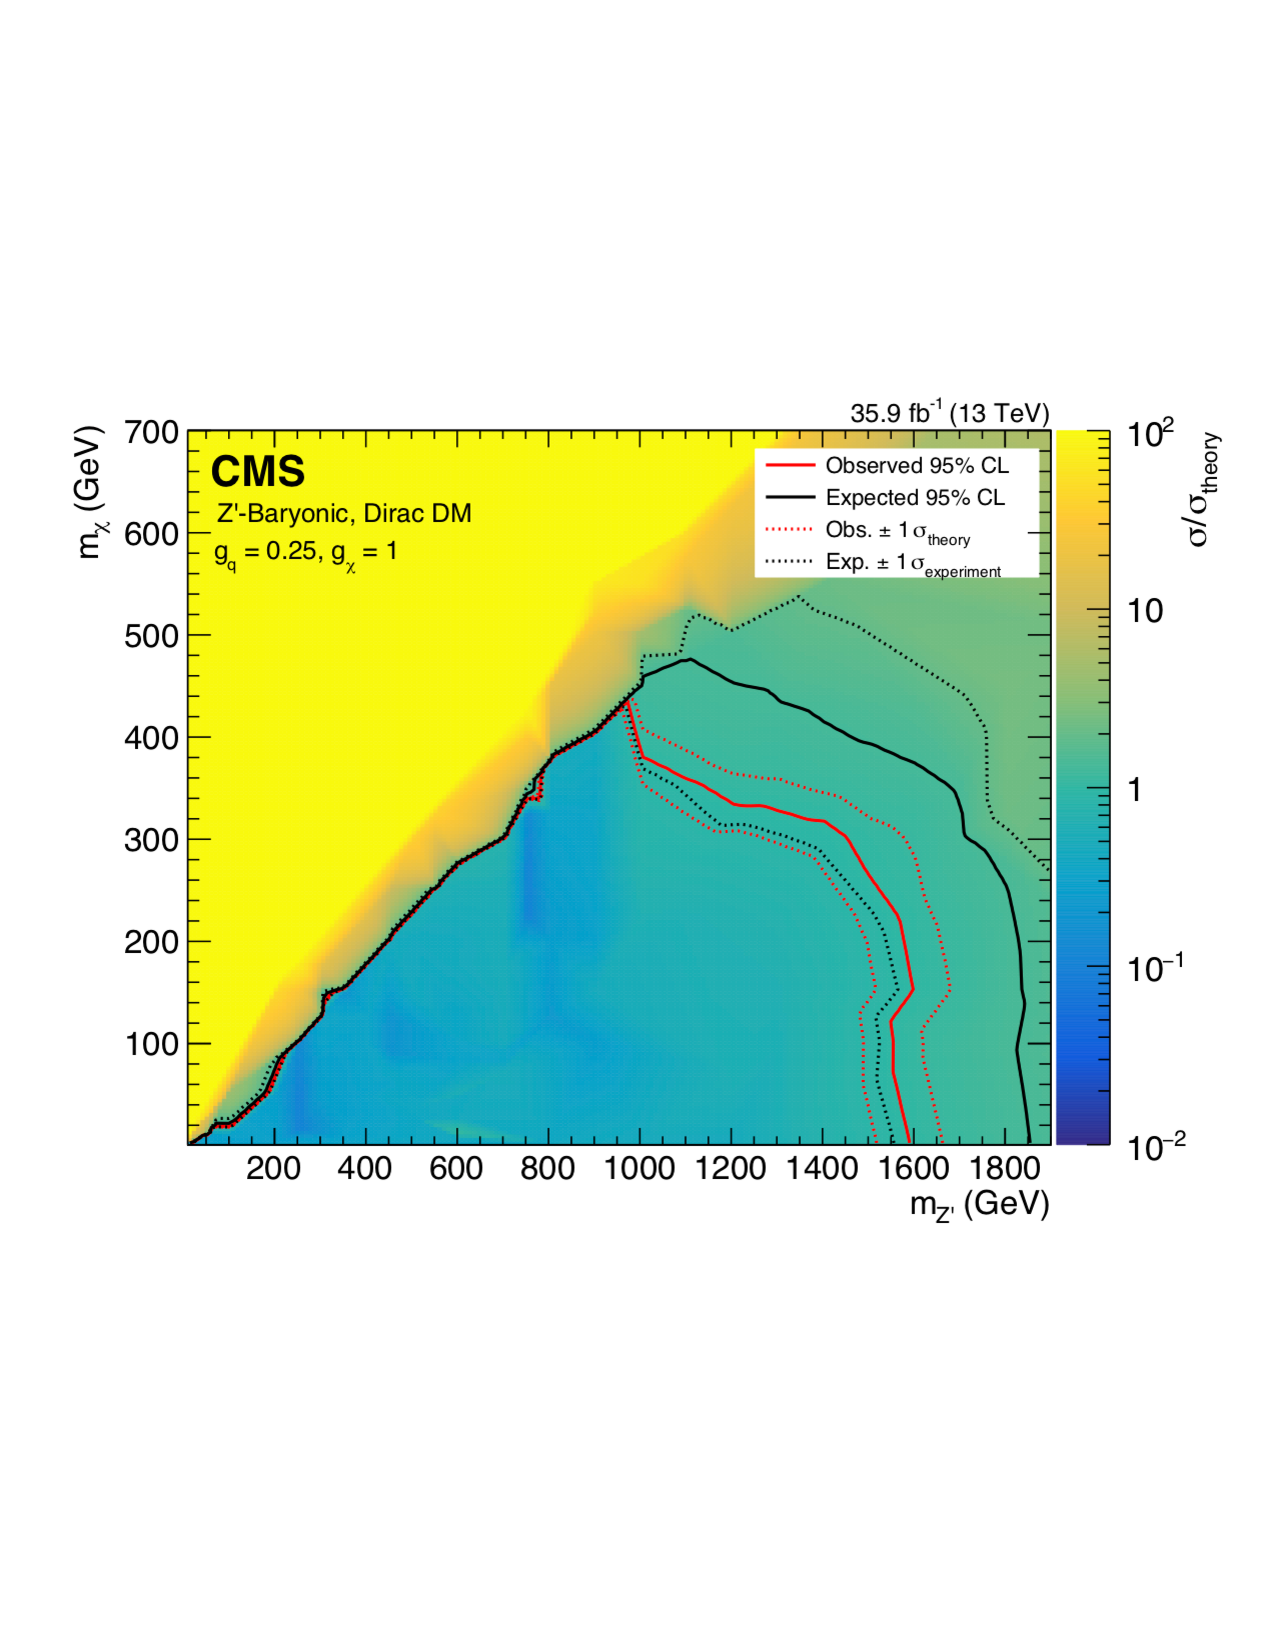
\includegraphics[width=0.475\textwidth]{figures/limits/limit2d_zpb_monohbb_.pdf}
  \caption{Upper limits on the signal strength modifier for the Baryonic Z' model (left). Mediators of up to 1.45\TeV are excluded for a DM mass of 1\GeV. Masses of the DM particle itself are excluded up to 230\GeV for a Z' mass of 1.25\TeV.}
  \label{fig:limits}
\end{figure}




Figure~\ref{fig:limits} shows the expected and observed exclusion range as a function of $m_{\text{Z}'}$ and $m_{\chi}$ for the Baryonic Z' model. For a DM mass of 1\GeV, masses $\mzp<1.6\TeV$ are excluded. The expected exclusion boundary is 1.85\TeV. Masses for the DM particles of up to 475\GeV are excluded for a 1.1\TeV Z' mass. These are the most stringent limits on this model so far. %These results can be turned into limits on the spin-independent cross section, see $-$FIG XX$-$. 

To compare results with DM direct detection experiments limits from the Baryonic Z' model are converted in terms of spin-indepedent (SI)cross section \SigSI for DM scattering off a nucleus.
Following the recommendation of Ref.~\cite{presentDM} the value of $\sigma_\text{SI}$ is determined by the equation:

\begin{equation}
\sigma_\text{SI} = \frac{f^2(g_{\cPq})g^2_{\mathrm{DM}}\mu^2_{\mathrm{n}\chi}}{\pi m^4_{\mathrm{med}}},
\end{equation}

where $\mu_{\mathrm{n}\chi}$ is the reduced mass of the DM-nucleon system and $f(g_{\cPq})$ is the mediator-nucleon coupling, which is dependent on $g_{\cPq}$.
The resulting \SigSI limits as a function of DM mass are shown in Figure~\ref{fig:limitsdd}.
%Exclusions from several direct detection experiments are compared to our result.
Under the assumptions made for the Baryonic Z' model, limits are the most stringent for $m_\chi < 5\GeV$.


\begin{figure}
  \centering
%  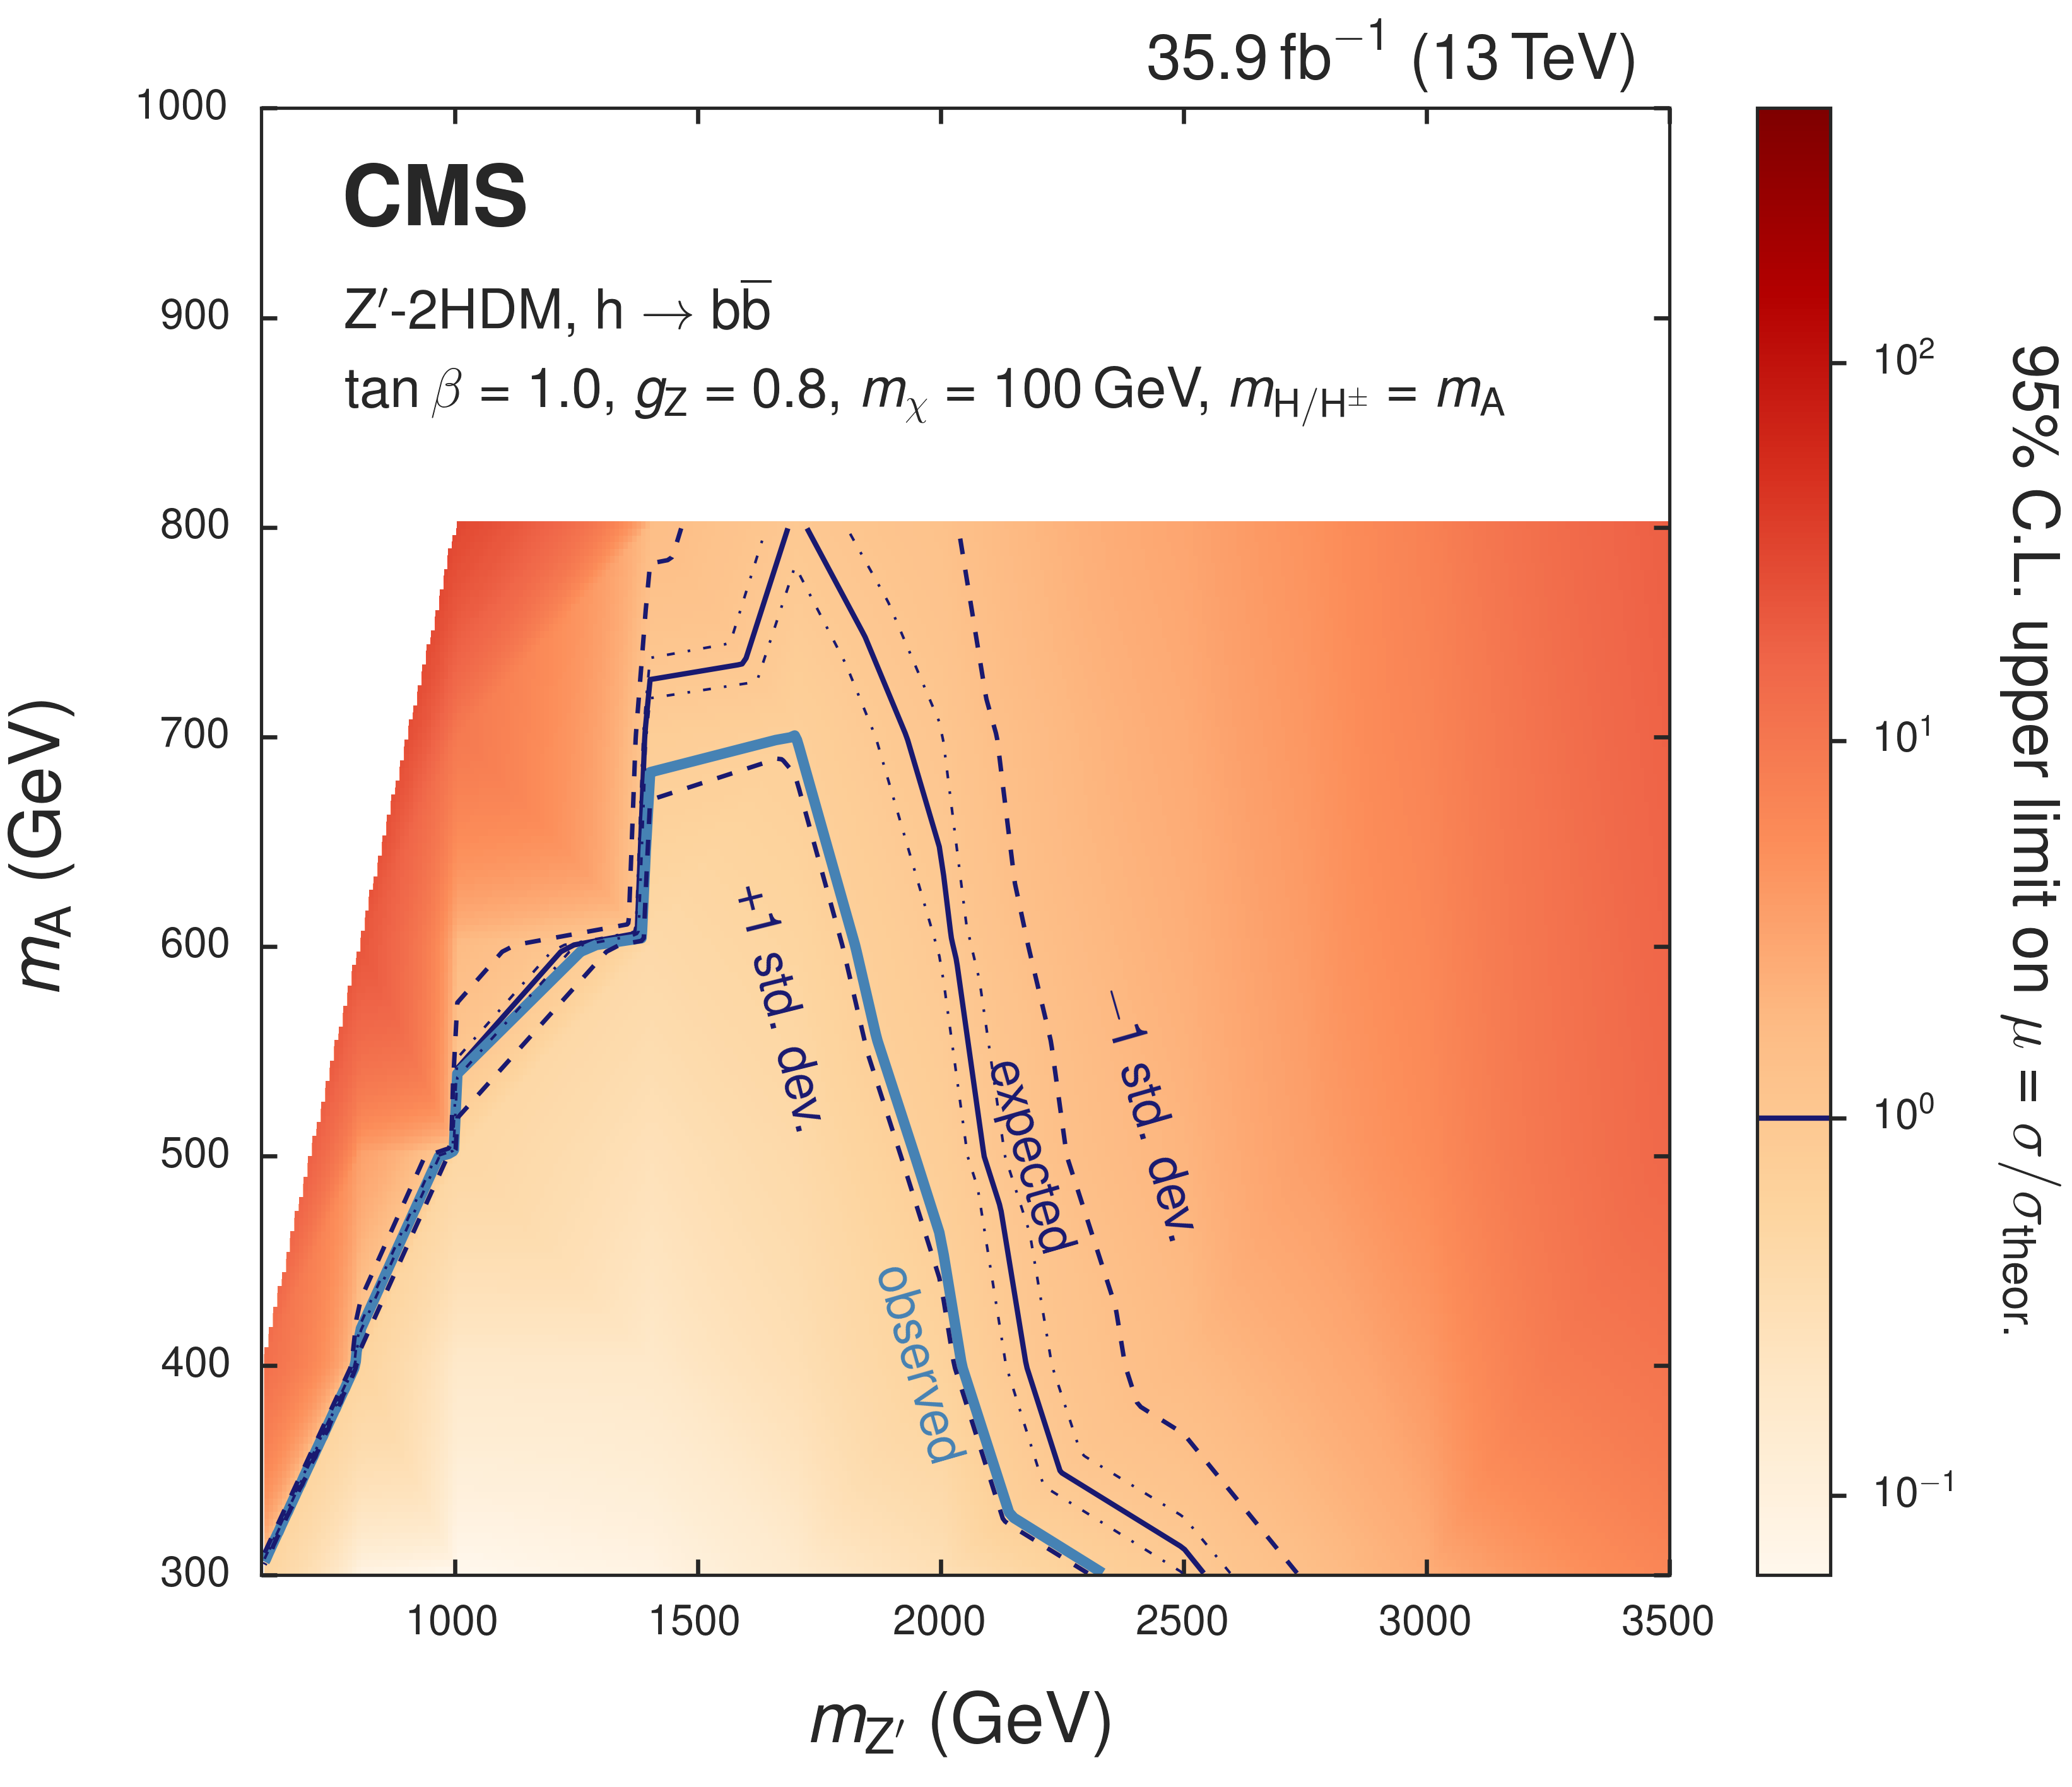
\includegraphics[width=0.475\textwidth]{figures/limits/limits_2hdm2d.png}
%  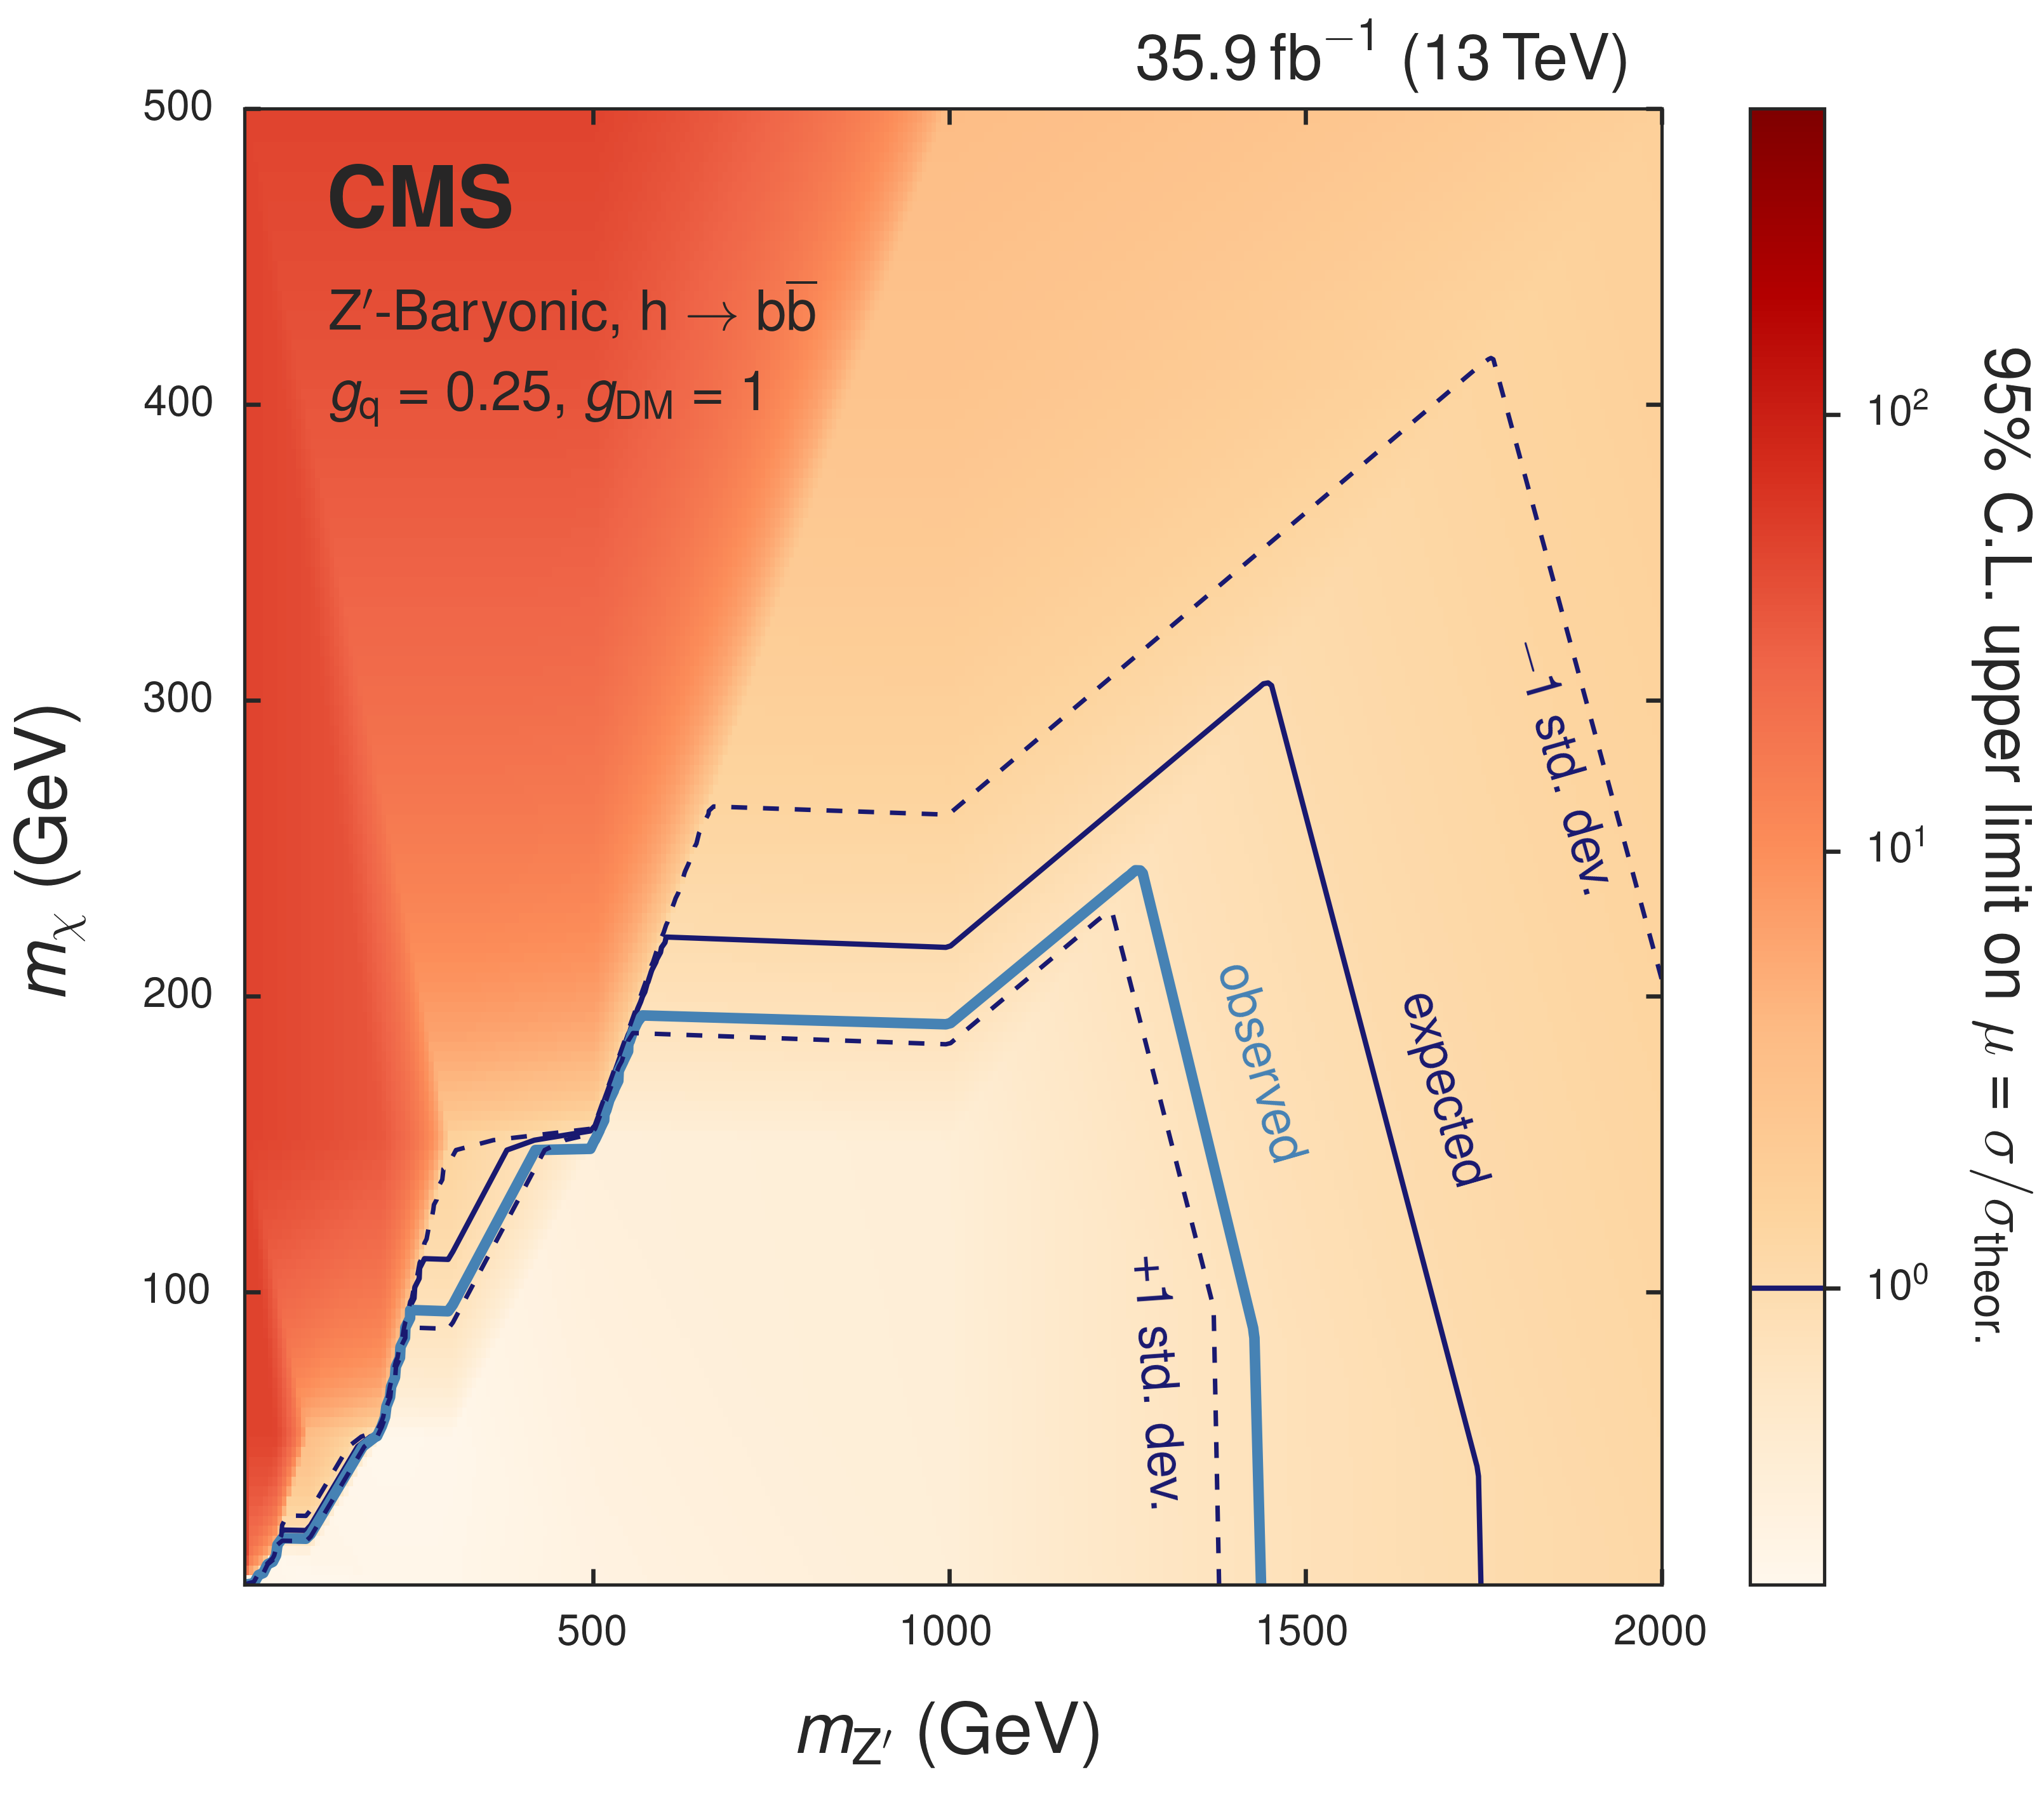
\includegraphics[width=0.475\textwidth]{figures/limits/limits_barzp2d.png}
  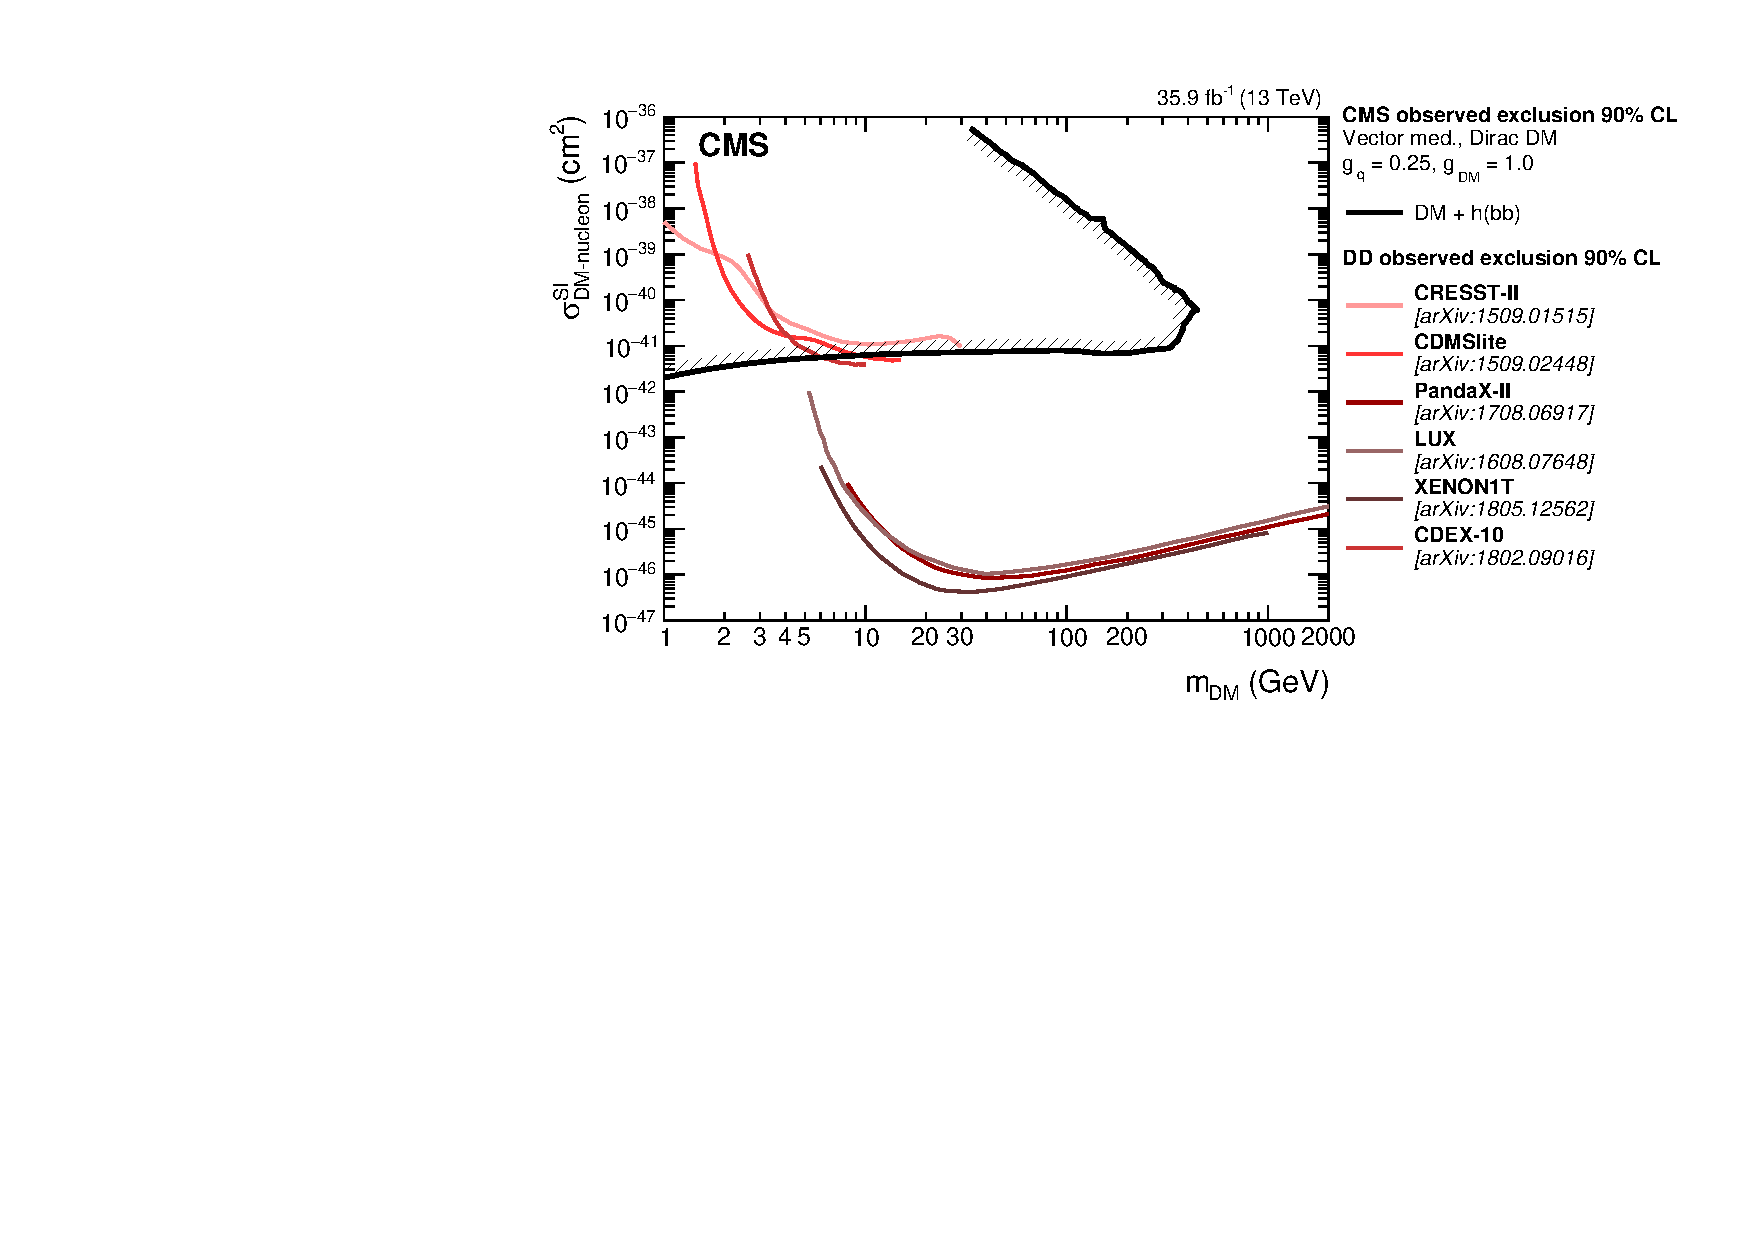
\includegraphics[width=0.775\textwidth]{figures/limits/SpinIndepend_XsecDM_MonoHbb_bb_obs_Summary.pdf}
  \caption{The 90\% \CL exclusion limits on the DM-nucleon SI scattering cross section as a function of $m_\chi$. 
Results obtained in this analysis are compared with those from a selection of direct detection (DD) experiments. 
The latter exclude the regions above the curves. 
Limits from CDMSLite~\cite{CDMSLite}, LUX~\cite{LUX}, XENON-1T~\cite{XENON1T}, PandaX-II~\cite{PandaxII}, and CRESST-II~\cite{CresstII} are shown.}
  \label{fig:limitsdd}
\end{figure}


\section{Summary}

A search for the associated production of DM particles with a Higgs
boson decaying into a b-quark pair is presented. No significant
deviation from the predictions of the SM is observed, and upper limits on
the production cross section predicted by the 2HDM+a model and the
Baryonic Z' model are established. They constitute the  most stringent  exclusions placed on the parameters in these
models so far. For the nominal choice of the mixing angle $\sin\theta$
and $\tan\beta$ in the 2HDM+a model, the search is able to exclude masses
$500<m_\text{A}<900\GeV$ assuming $m_\text{a}=150\GeV$. Scanning over
$\sin\theta$ for two example benchmark points, we exclude
$0.35<\sin\theta<0.75$ for $m_\text{A}=600\GeV$ and
$m_\text{a}=200\GeV$.  Finally, $\tan\beta$ values between 0.5 and 2.0
(1.6) are excluded for $m_\text{A}=600\GeV$ and $m_\text{a}=100$
(150)\GeV. In all 2HDM+a interpretations, a DM mass of $m_\chi=10\GeV$ is assumed. For the Baryonic Z' model, we exclude Z' masses up to 1.6\TeV for a DM mass of 1\GeV, and DM masses up to 475\GeV for a Z' mass of 1.1\TeV. Reinterpreting the results for the Baryonic Z' model under the assumption of an $s$-channel simplified DM model results in a higher sensitivity of the search presented compared to direct detection experiments for $m_\chi<5\GeV$. 

 
